\documentclass[1p]{elsarticle_modified}
%\bibliographystyle{elsarticle-num}

%\usepackage[colorlinks]{hyperref}
%\usepackage{abbrmath_seonhwa} %\Abb, \Ascr, \Acal ,\Abf, \Afrak
\usepackage{amsfonts}
\usepackage{amssymb}
\usepackage{amsmath}
\usepackage{amsthm}
\usepackage{scalefnt}
\usepackage{amsbsy}
\usepackage{kotex}
\usepackage{caption}
\usepackage{subfig}
\usepackage{color}
\usepackage{graphicx}
\usepackage{xcolor} %% white, black, red, green, blue, cyan, magenta, yellow
\usepackage{float}
\usepackage{setspace}
\usepackage{hyperref}

\usepackage{tikz}
\usetikzlibrary{arrows}

\usepackage{multirow}
\usepackage{array} % fixed length table
\usepackage{hhline}

%%%%%%%%%%%%%%%%%%%%%
\makeatletter
\renewcommand*\env@matrix[1][\arraystretch]{%
	\edef\arraystretch{#1}%
	\hskip -\arraycolsep
	\let\@ifnextchar\new@ifnextchar
	\array{*\c@MaxMatrixCols c}}
\makeatother %https://tex.stackexchange.com/questions/14071/how-can-i-increase-the-line-spacing-in-a-matrix
%%%%%%%%%%%%%%%

\usepackage[normalem]{ulem}

\newcommand{\msout}[1]{\ifmmode\text{\sout{\ensuremath{#1}}}\else\sout{#1}\fi}
%SOURCE: \msout is \stkout macro in https://tex.stackexchange.com/questions/20609/strikeout-in-math-mode

\newcommand{\cancel}[1]{
	\ifmmode
	{\color{red}\msout{#1}}
	\else
	{\color{red}\sout{#1}}
	\fi
}

\newcommand{\add}[1]{
	{\color{blue}\uwave{#1}}
}

\newcommand{\replace}[2]{
	\ifmmode
	{\color{red}\msout{#1}}{\color{blue}\uwave{#2}}
	\else
	{\color{red}\sout{#1}}{\color{blue}\uwave{#2}}
	\fi
}

\newcommand{\Sol}{\mathcal{S}} %segment
\newcommand{\D}{D} %diagram
\newcommand{\A}{\mathcal{A}} %arc


%%%%%%%%%%%%%%%%%%%%%%%%%%%%%5 test

\def\sl{\operatorname{\textup{SL}}(2,\Cbb)}
\def\psl{\operatorname{\textup{PSL}}(2,\Cbb)}
\def\quan{\mkern 1mu \triangleright \mkern 1mu}

\theoremstyle{definition}
\newtheorem{thm}{Theorem}[section]
\newtheorem{prop}[thm]{Proposition}
\newtheorem{lem}[thm]{Lemma}
\newtheorem{ques}[thm]{Question}
\newtheorem{cor}[thm]{Corollary}
\newtheorem{defn}[thm]{Definition}
\newtheorem{exam}[thm]{Example}
\newtheorem{rmk}[thm]{Remark}
\newtheorem{alg}[thm]{Algorithm}

\newcommand{\I}{\sqrt{-1}}
\begin{document}

%\begin{frontmatter}
%
%\title{Boundary parabolic representations of knots up to 8 crossings}
%
%%% Group authors per affiliation:
%\author{Yunhi Cho} 
%\address{Department of Mathematics, University of Seoul, Seoul, Korea}
%\ead{yhcho@uos.ac.kr}
%
%
%\author{Seonhwa Kim} %\fnref{s_kim}}
%\address{Center for Geometry and Physics, Institute for Basic Science, Pohang, 37673, Korea}
%\ead{ryeona17@ibs.re.kr}
%
%\author{Hyuk Kim}
%\address{Department of Mathematical Sciences, Seoul National University, Seoul 08826, Korea}
%\ead{hyukkim@snu.ac.kr}
%
%\author{Seokbeom Yoon}
%\address{Department of Mathematical Sciences, Seoul National University, Seoul, 08826,  Korea}
%\ead{sbyoon15@snu.ac.kr}
%
%\begin{abstract}
%We find all boundary parabolic representation of knots up to 8 crossings.
%
%\end{abstract}
%\begin{keyword}
%    \MSC[2010] 57M25 
%\end{keyword}
%
%\end{frontmatter}

%\linenumbers
%\tableofcontents
%
\newcommand\colored[1]{\textcolor{white}{\rule[-0.35ex]{0.8em}{1.4ex}}\kern-0.8em\color{red} #1}%
%\newcommand\colored[1]{\textcolor{white}{ #1}\kern-2.17ex	\textcolor{white}{ #1}\kern-1.81ex	\textcolor{white}{ #1}\kern-2.15ex\color{red}#1	}

{\Large $\underline{12a_{0963}~(K12a_{0963})}$}

\setlength{\tabcolsep}{10pt}
\renewcommand{\arraystretch}{1.6}
\vspace{1cm}\begin{tabular}{m{100pt}>{\centering\arraybackslash}m{274pt}}
\multirow{5}{120pt}{
	\centering
	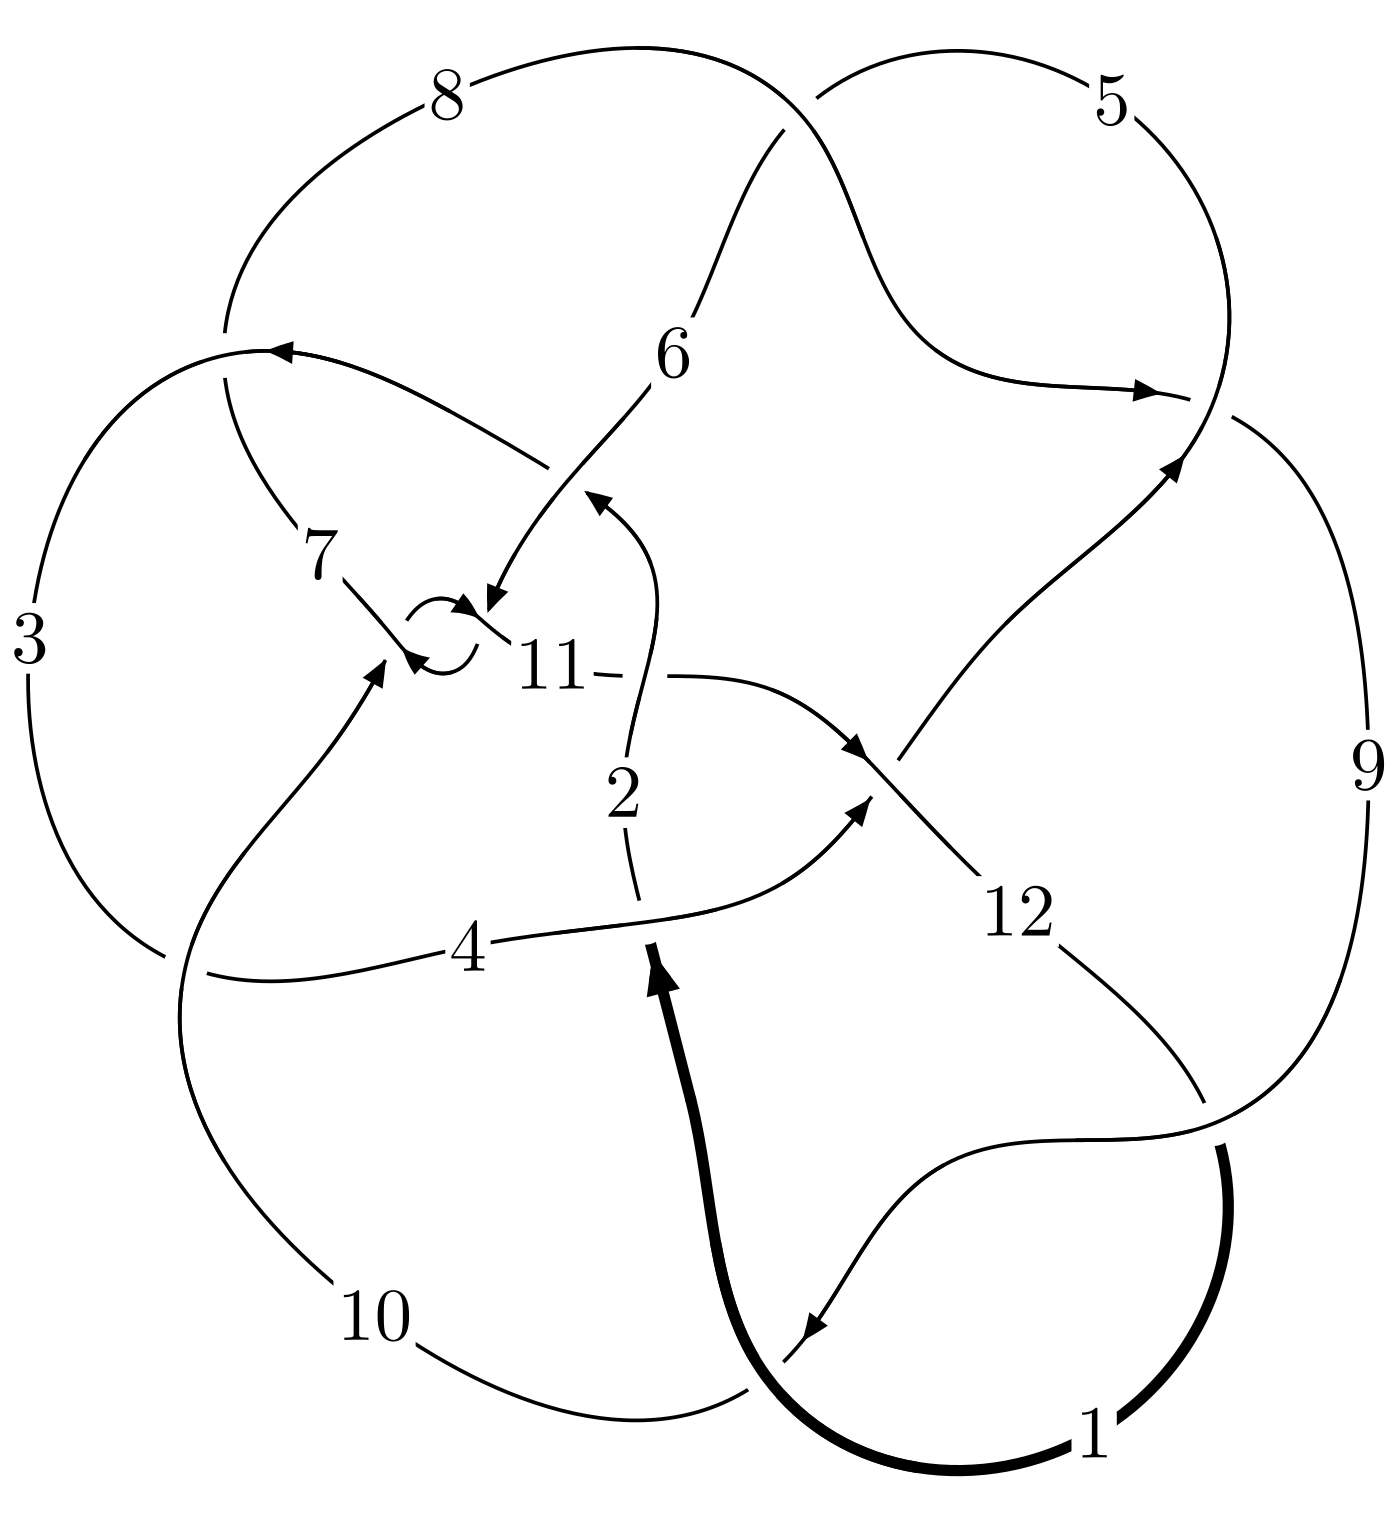
\includegraphics[width=112pt]{../../../GIT/diagram.site/Diagrams/png/1764_12a_0963.png}\\
\ \ \ A knot diagram\footnotemark}&
\allowdisplaybreaks
\textbf{Linearized knot diagam} \\
\cline{2-2}
 &
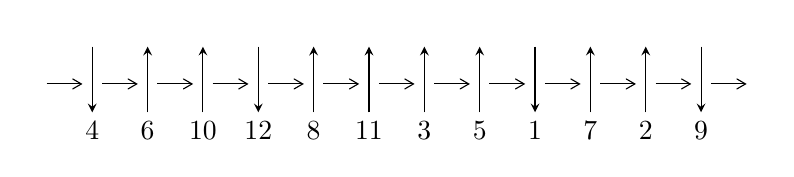
\begin{tikzpicture}[x=20pt, y=17pt]
	% nodes
	\node (C0) at (0, 0) {};
	\node (C1) at (1, 0) {};
	\node (C1U) at (1, +1) {};
	\node (C1D) at (1, -1) {4};

	\node (C2) at (2, 0) {};
	\node (C2U) at (2, +1) {};
	\node (C2D) at (2, -1) {6};

	\node (C3) at (3, 0) {};
	\node (C3U) at (3, +1) {};
	\node (C3D) at (3, -1) {10};

	\node (C4) at (4, 0) {};
	\node (C4U) at (4, +1) {};
	\node (C4D) at (4, -1) {12};

	\node (C5) at (5, 0) {};
	\node (C5U) at (5, +1) {};
	\node (C5D) at (5, -1) {8};

	\node (C6) at (6, 0) {};
	\node (C6U) at (6, +1) {};
	\node (C6D) at (6, -1) {11};

	\node (C7) at (7, 0) {};
	\node (C7U) at (7, +1) {};
	\node (C7D) at (7, -1) {3};

	\node (C8) at (8, 0) {};
	\node (C8U) at (8, +1) {};
	\node (C8D) at (8, -1) {5};

	\node (C9) at (9, 0) {};
	\node (C9U) at (9, +1) {};
	\node (C9D) at (9, -1) {1};

	\node (C10) at (10, 0) {};
	\node (C10U) at (10, +1) {};
	\node (C10D) at (10, -1) {7};

	\node (C11) at (11, 0) {};
	\node (C11U) at (11, +1) {};
	\node (C11D) at (11, -1) {2};

	\node (C12) at (12, 0) {};
	\node (C12U) at (12, +1) {};
	\node (C12D) at (12, -1) {9};
	\node (C13) at (13, 0) {};

	% arrows
	\draw[->,>={angle 60}]
	(C0) edge (C1) (C1) edge (C2) (C2) edge (C3) (C3) edge (C4) (C4) edge (C5) (C5) edge (C6) (C6) edge (C7) (C7) edge (C8) (C8) edge (C9) (C9) edge (C10) (C10) edge (C11) (C11) edge (C12) (C12) edge (C13) ;	\draw[->,>=stealth]
	(C1U) edge (C1D) (C2D) edge (C2U) (C3D) edge (C3U) (C4U) edge (C4D) (C5D) edge (C5U) (C6D) edge (C6U) (C7D) edge (C7U) (C8D) edge (C8U) (C9U) edge (C9D) (C10D) edge (C10U) (C11D) edge (C11U) (C12U) edge (C12D) ;
	\end{tikzpicture} \\
\hhline{~~} \\& 
\textbf{Solving Sequence} \\ \cline{2-2} 
 &
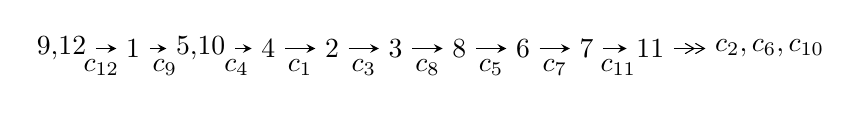
\begin{tikzpicture}[x=23pt, y=7pt]
	% node
	\node (A0) at (-1/8, 0) {9,12};
	\node (A1) at (1, 0) {1};
	\node (A2) at (33/16, 0) {5,10};
	\node (A3) at (25/8, 0) {4};
	\node (A4) at (33/8, 0) {2};
	\node (A5) at (41/8, 0) {3};
	\node (A6) at (49/8, 0) {8};
	\node (A7) at (57/8, 0) {6};
	\node (A8) at (65/8, 0) {7};
	\node (A9) at (73/8, 0) {11};
	\node (C1) at (1/2, -1) {$c_{12}$};
	\node (C2) at (3/2, -1) {$c_{9}$};
	\node (C3) at (21/8, -1) {$c_{4}$};
	\node (C4) at (29/8, -1) {$c_{1}$};
	\node (C5) at (37/8, -1) {$c_{3}$};
	\node (C6) at (45/8, -1) {$c_{8}$};
	\node (C7) at (53/8, -1) {$c_{5}$};
	\node (C8) at (61/8, -1) {$c_{7}$};
	\node (C9) at (69/8, -1) {$c_{11}$};
	\node (A10) at (11, 0) {$c_{2},c_{6},c_{10}$};

	% edge
	\draw[->,>=stealth]	
	(A0) edge (A1) (A1) edge (A2) (A2) edge (A3) (A3) edge (A4) (A4) edge (A5) (A5) edge (A6) (A6) edge (A7) (A7) edge (A8) (A8) edge (A9) ;
	\draw[->>,>={angle 60}]	
	(A9) edge (A10);
\end{tikzpicture} \\ 

\end{tabular} \\

\footnotetext{
The image of knot diagram is generated by the software ``\textbf{Draw programme}" developed by Andrew Bartholomew(\url{http://www.layer8.co.uk/maths/draw/index.htm\#Running-draw}), where we modified some parts for our purpose(\url{https://github.com/CATsTAILs/LinksPainter}).
}\phantom \\ \newline 
\centering \textbf{Ideals for irreducible components\footnotemark of $X_{\text{par}}$} 
 
\begin{align*}
I^u_{1}&=\langle 
3.25168\times10^{823} u^{156}-2.59445\times10^{823} u^{155}+\cdots+7.76883\times10^{823} b-4.79193\times10^{825},\\
\phantom{I^u_{1}}&\phantom{= \langle  }-3.11599\times10^{825} u^{156}+2.47642\times10^{825} u^{155}+\cdots+1.40616\times10^{826} a+5.05878\times10^{827},\\
\phantom{I^u_{1}}&\phantom{= \langle  }u^{157}-2 u^{156}+\cdots-1089 u+181\rangle \\
I^u_{2}&=\langle 
1.92631\times10^{42} u^{46}-3.43494\times10^{42} u^{45}+\cdots+7.75734\times10^{42} b+1.10349\times10^{43},\\
\phantom{I^u_{2}}&\phantom{= \langle  }-2.95227\times10^{43} u^{46}+3.11133\times10^{43} u^{45}+\cdots+5.43014\times10^{43} a-9.32130\times10^{43},\;u^{47}- u^{46}+\cdots+8 u+7\rangle \\
\\
\end{align*}
\raggedright * 2 irreducible components of $\dim_{\mathbb{C}}=0$, with total 204 representations.\\
\footnotetext{All coefficients of polynomials are rational numbers. But the coefficients are sometimes approximated in decimal forms when there is not enough margin.}
\newpage
\renewcommand{\arraystretch}{1}
\centering \section*{I. $I^u_{1}= \langle 3.25\times10^{823} u^{156}-2.59\times10^{823} u^{155}+\cdots+7.77\times10^{823} b-4.79\times10^{825},\;-3.12\times10^{825} u^{156}+2.48\times10^{825} u^{155}+\cdots+1.41\times10^{826} a+5.06\times10^{827},\;u^{157}-2 u^{156}+\cdots-1089 u+181 \rangle$}
\flushleft \textbf{(i) Arc colorings}\\
\begin{tabular}{m{7pt} m{180pt} m{7pt} m{180pt} }
\flushright $a_{9}=$&$\begin{pmatrix}0\\u\end{pmatrix}$ \\
\flushright $a_{12}=$&$\begin{pmatrix}1\\0\end{pmatrix}$ \\
\flushright $a_{1}=$&$\begin{pmatrix}1\\u^2\end{pmatrix}$ \\
\flushright $a_{5}=$&$\begin{pmatrix}0.221596 u^{156}-0.176112 u^{155}+\cdots+213.321 u-35.9759\\-0.418554 u^{156}+0.333957 u^{155}+\cdots-317.116 u+61.6815\end{pmatrix}$ \\
\flushright $a_{10}=$&$\begin{pmatrix}- u\\- u^3+u\end{pmatrix}$ \\
\flushright $a_{4}=$&$\begin{pmatrix}-0.196958 u^{156}+0.157845 u^{155}+\cdots-103.794 u+25.7056\\-0.418554 u^{156}+0.333957 u^{155}+\cdots-317.116 u+61.6815\end{pmatrix}$ \\
\flushright $a_{2}=$&$\begin{pmatrix}0.178853 u^{156}-0.188599 u^{155}+\cdots+119.981 u-39.6455\\-0.0623607 u^{156}+0.0472106 u^{155}+\cdots-53.5035 u+12.0020\end{pmatrix}$ \\
\flushright $a_{3}=$&$\begin{pmatrix}0.268823 u^{156}-0.214033 u^{155}+\cdots+253.388 u-43.3447\\-0.205428 u^{156}+0.161209 u^{155}+\cdots-149.106 u+29.4286\end{pmatrix}$ \\
\flushright $a_{8}=$&$\begin{pmatrix}0.173692 u^{156}-0.162984 u^{155}+\cdots+150.878 u-32.2694\\0.0543462 u^{156}-0.0363523 u^{155}+\cdots+29.2802 u-2.81016\end{pmatrix}$ \\
\flushright $a_{6}=$&$\begin{pmatrix}-0.231849 u^{156}+0.226710 u^{155}+\cdots-264.361 u+53.3549\\0.109896 u^{156}-0.0881361 u^{155}+\cdots+89.3275 u-19.1200\end{pmatrix}$ \\
\flushright $a_{7}=$&$\begin{pmatrix}-0.00668521 u^{156}-0.000568235 u^{155}+\cdots+25.5452 u-11.8966\\0.0533812 u^{156}-0.0363507 u^{155}+\cdots+48.9661 u-5.83195\end{pmatrix}$ \\
\flushright $a_{11}=$&$\begin{pmatrix}0.0294108 u^{156}-0.0135338 u^{155}+\cdots+12.9035 u+6.64770\\0.117190 u^{156}-0.0887343 u^{155}+\cdots+86.4006 u-17.0782\end{pmatrix}$\\&\end{tabular}
\flushleft \textbf{(ii) Obstruction class $= -1$}\\~\\
\flushleft \textbf{(iii) Cusp Shapes $= 0.205349 u^{156}-0.170433 u^{155}+\cdots+170.257 u-38.4072$}\\~\\
\newpage\renewcommand{\arraystretch}{1}
\flushleft \textbf{(iv) u-Polynomials at the component}\newline \\
\begin{tabular}{m{50pt}|m{274pt}}
Crossings & \hspace{64pt}u-Polynomials at each crossing \\
\hline $$\begin{aligned}c_{1}\end{aligned}$$&$\begin{aligned}
&u^{157}+5 u^{156}+\cdots+11551514 u-666271
\end{aligned}$\\
\hline $$\begin{aligned}c_{2}\end{aligned}$$&$\begin{aligned}
&u^{157}- u^{156}+\cdots-1628098428 u-107670653
\end{aligned}$\\
\hline $$\begin{aligned}c_{3}\end{aligned}$$&$\begin{aligned}
&u^{157}+u^{156}+\cdots-6882417969378 u-579271043533
\end{aligned}$\\
\hline $$\begin{aligned}c_{4}\end{aligned}$$&$\begin{aligned}
&u^{157}-37 u^{155}+\cdots+445344963 u-17796191
\end{aligned}$\\
\hline $$\begin{aligned}c_{5},c_{8}\end{aligned}$$&$\begin{aligned}
&u^{157}+10 u^{156}+\cdots-968 u-181
\end{aligned}$\\
\hline $$\begin{aligned}c_{6},c_{10}\end{aligned}$$&$\begin{aligned}
&u^{157}-3 u^{156}+\cdots+7 u-1
\end{aligned}$\\
\hline $$\begin{aligned}c_{7}\end{aligned}$$&$\begin{aligned}
&u^{157}+38 u^{155}+\cdots+132651545 u-435199883
\end{aligned}$\\
\hline $$\begin{aligned}c_{9},c_{12}\end{aligned}$$&$\begin{aligned}
&u^{157}+2 u^{156}+\cdots-1089 u-181
\end{aligned}$\\
\hline $$\begin{aligned}c_{11}\end{aligned}$$&$\begin{aligned}
&u^{157}+12 u^{156}+\cdots+844976503738 u+47066586319
\end{aligned}$\\
\hline
\end{tabular}\\~\\
\newpage\renewcommand{\arraystretch}{1}
\flushleft \textbf{(v) Riley Polynomials at the component}\newline \\
\begin{tabular}{m{50pt}|m{274pt}}
Crossings & \hspace{64pt}Riley Polynomials at each crossing \\
\hline $$\begin{aligned}c_{1}\end{aligned}$$&$\begin{aligned}
&y^{157}-49 y^{156}+\cdots+104808094653642 y-443917045441
\end{aligned}$\\
\hline $$\begin{aligned}c_{2}\end{aligned}$$&$\begin{aligned}
&y^{157}+59 y^{156}+\cdots-404534046342627964 y-11592969517446409
\end{aligned}$\\
\hline $$\begin{aligned}c_{3}\end{aligned}$$&$\begin{aligned}
&y^{157}+111 y^{156}+\cdots-4.36\times10^{24} y-3.36\times10^{23}
\end{aligned}$\\
\hline $$\begin{aligned}c_{4}\end{aligned}$$&$\begin{aligned}
&y^{157}-74 y^{156}+\cdots+112157843337933533 y-316704414108481
\end{aligned}$\\
\hline $$\begin{aligned}c_{5},c_{8}\end{aligned}$$&$\begin{aligned}
&y^{157}+150 y^{156}+\cdots+9673532 y-32761
\end{aligned}$\\
\hline $$\begin{aligned}c_{6},c_{10}\end{aligned}$$&$\begin{aligned}
&y^{157}+111 y^{156}+\cdots+165 y-1
\end{aligned}$\\
\hline $$\begin{aligned}c_{7}\end{aligned}$$&$\begin{aligned}
&y^{157}+76 y^{156}+\cdots-801491013938418801 y-189398938163213689
\end{aligned}$\\
\hline $$\begin{aligned}c_{9},c_{12}\end{aligned}$$&$\begin{aligned}
&y^{157}-118 y^{156}+\cdots+1444751 y-32761
\end{aligned}$\\
\hline $$\begin{aligned}c_{11}\end{aligned}$$&$\begin{aligned}
&y^{157}+84 y^{156}+\cdots+1.62\times10^{22} y-2.22\times10^{21}
\end{aligned}$\\
\hline
\end{tabular}\\~\\
\newpage\flushleft \textbf{(vi) Complex Volumes and Cusp Shapes}
$$\begin{array}{c|c|c}  
\text{Solutions to }I^u_{1}& \I (\text{vol} + \sqrt{-1}CS) & \text{Cusp shape}\\
 \hline 
\begin{aligned}
u &= \phantom{-}0.911310 + 0.293013 I \\
a &= \phantom{-}0.422959 - 0.500306 I \\
b &= \phantom{-}0.675145 + 0.486620 I\end{aligned}
 & -1.96969 - 1.58228 I & \phantom{-0.000000 } 0 \\ \hline\begin{aligned}
u &= \phantom{-}0.911310 - 0.293013 I \\
a &= \phantom{-}0.422959 + 0.500306 I \\
b &= \phantom{-}0.675145 - 0.486620 I\end{aligned}
 & -1.96969 + 1.58228 I & \phantom{-0.000000 } 0 \\ \hline\begin{aligned}
u &= -0.387840 + 0.973856 I \\
a &= -1.200220 + 0.398785 I \\
b &= \phantom{-}1.255970 + 0.451783 I\end{aligned}
 & -5.67139 - 4.88778 I & \phantom{-0.000000 } 0 \\ \hline\begin{aligned}
u &= -0.387840 - 0.973856 I \\
a &= -1.200220 - 0.398785 I \\
b &= \phantom{-}1.255970 - 0.451783 I\end{aligned}
 & -5.67139 + 4.88778 I & \phantom{-0.000000 } 0 \\ \hline\begin{aligned}
u &= -1.058010 + 0.108048 I \\
a &= \phantom{-}1.078700 - 0.213102 I \\
b &= \phantom{-}0.635902 - 0.081974 I\end{aligned}
 & \phantom{-}0.108417 + 0.376808 I & \phantom{-0.000000 } 0 \\ \hline\begin{aligned}
u &= -1.058010 - 0.108048 I \\
a &= \phantom{-}1.078700 + 0.213102 I \\
b &= \phantom{-}0.635902 + 0.081974 I\end{aligned}
 & \phantom{-}0.108417 - 0.376808 I & \phantom{-0.000000 } 0 \\ \hline\begin{aligned}
u &= \phantom{-}1.062930 + 0.087493 I \\
a &= -0.704856 + 0.159930 I \\
b &= -1.22300 - 0.79175 I\end{aligned}
 & -1.27458 - 1.99100 I & \phantom{-0.000000 } 0 \\ \hline\begin{aligned}
u &= \phantom{-}1.062930 - 0.087493 I \\
a &= -0.704856 - 0.159930 I \\
b &= -1.22300 + 0.79175 I\end{aligned}
 & -1.27458 + 1.99100 I & \phantom{-0.000000 } 0 \\ \hline\begin{aligned}
u &= -1.059890 + 0.177175 I \\
a &= -0.232872 - 1.389900 I \\
b &= -0.959988 + 0.026640 I\end{aligned}
 & -7.39949 - 1.96456 I & \phantom{-0.000000 } 0 \\ \hline\begin{aligned}
u &= -1.059890 - 0.177175 I \\
a &= -0.232872 + 1.389900 I \\
b &= -0.959988 - 0.026640 I\end{aligned}
 & -7.39949 + 1.96456 I & \phantom{-0.000000 } 0\\
 \hline 
 \end{array}$$\newpage$$\begin{array}{c|c|c}  
\text{Solutions to }I^u_{1}& \I (\text{vol} + \sqrt{-1}CS) & \text{Cusp shape}\\
 \hline 
\begin{aligned}
u &= \phantom{-}0.285052 + 1.070700 I \\
a &= -1.116590 - 0.322100 I \\
b &= \phantom{-}0.904472 + 0.446905 I\end{aligned}
 & -3.72967 - 2.43277 I & \phantom{-0.000000 } 0 \\ \hline\begin{aligned}
u &= \phantom{-}0.285052 - 1.070700 I \\
a &= -1.116590 + 0.322100 I \\
b &= \phantom{-}0.904472 - 0.446905 I\end{aligned}
 & -3.72967 + 2.43277 I & \phantom{-0.000000 } 0 \\ \hline\begin{aligned}
u &= -1.083450 + 0.247951 I \\
a &= -0.644397 - 0.231290 I \\
b &= -1.34277 + 0.53989 I\end{aligned}
 & -3.56097 + 6.59812 I & \phantom{-0.000000 } 0 \\ \hline\begin{aligned}
u &= -1.083450 - 0.247951 I \\
a &= -0.644397 + 0.231290 I \\
b &= -1.34277 - 0.53989 I\end{aligned}
 & -3.56097 - 6.59812 I & \phantom{-0.000000 } 0 \\ \hline\begin{aligned}
u &= -0.071448 + 0.876093 I \\
a &= \phantom{-}0.807592 + 0.554786 I \\
b &= -0.542808 - 0.487692 I\end{aligned}
 & \phantom{-}1.65200 - 2.03206 I & \phantom{-0.000000 } 0 \\ \hline\begin{aligned}
u &= -0.071448 - 0.876093 I \\
a &= \phantom{-}0.807592 - 0.554786 I \\
b &= -0.542808 + 0.487692 I\end{aligned}
 & \phantom{-}1.65200 + 2.03206 I & \phantom{-0.000000 } 0 \\ \hline\begin{aligned}
u &= \phantom{-}0.025069 + 0.871018 I \\
a &= \phantom{-}0.324040 - 1.093510 I \\
b &= -0.724981 + 0.867463 I\end{aligned}
 & -4.55498 + 8.98621 I & \phantom{-0.000000 } 0 \\ \hline\begin{aligned}
u &= \phantom{-}0.025069 - 0.871018 I \\
a &= \phantom{-}0.324040 + 1.093510 I \\
b &= -0.724981 - 0.867463 I\end{aligned}
 & -4.55498 - 8.98621 I & \phantom{-0.000000 } 0 \\ \hline\begin{aligned}
u &= \phantom{-}0.816425 + 0.301933 I \\
a &= \phantom{-}0.888162 + 0.435117 I \\
b &= \phantom{-}0.369688 + 0.168423 I\end{aligned}
 & -2.25118 + 2.07318 I & \phantom{-0.000000 } 0 \\ \hline\begin{aligned}
u &= \phantom{-}0.816425 - 0.301933 I \\
a &= \phantom{-}0.888162 - 0.435117 I \\
b &= \phantom{-}0.369688 - 0.168423 I\end{aligned}
 & -2.25118 - 2.07318 I & \phantom{-0.000000 } 0\\
 \hline 
 \end{array}$$\newpage$$\begin{array}{c|c|c}  
\text{Solutions to }I^u_{1}& \I (\text{vol} + \sqrt{-1}CS) & \text{Cusp shape}\\
 \hline 
\begin{aligned}
u &= -0.562324 + 0.663290 I \\
a &= \phantom{-}0.300737 + 0.551236 I \\
b &= \phantom{-}0.312522 - 0.887888 I\end{aligned}
 & -1.93889 + 2.36574 I & \phantom{-0.000000 } 0 \\ \hline\begin{aligned}
u &= -0.562324 - 0.663290 I \\
a &= \phantom{-}0.300737 - 0.551236 I \\
b &= \phantom{-}0.312522 + 0.887888 I\end{aligned}
 & -1.93889 - 2.36574 I & \phantom{-0.000000 } 0 \\ \hline\begin{aligned}
u &= \phantom{-}0.109075 + 0.850935 I \\
a &= \phantom{-}1.45809 + 0.06873 I \\
b &= -0.421659 + 0.344018 I\end{aligned}
 & -4.13875 - 0.45277 I & \phantom{-0.000000 } 0 \\ \hline\begin{aligned}
u &= \phantom{-}0.109075 - 0.850935 I \\
a &= \phantom{-}1.45809 - 0.06873 I \\
b &= -0.421659 - 0.344018 I\end{aligned}
 & -4.13875 + 0.45277 I & \phantom{-0.000000 } 0 \\ \hline\begin{aligned}
u &= \phantom{-}0.203065 + 0.818259 I \\
a &= \phantom{-}0.426590 - 0.467011 I \\
b &= -0.117108 + 0.690407 I\end{aligned}
 & \phantom{-}0.31892 - 2.30117 I & \phantom{-0.000000 } 0 \\ \hline\begin{aligned}
u &= \phantom{-}0.203065 - 0.818259 I \\
a &= \phantom{-}0.426590 + 0.467011 I \\
b &= -0.117108 - 0.690407 I\end{aligned}
 & \phantom{-}0.31892 + 2.30117 I & \phantom{-0.000000 } 0 \\ \hline\begin{aligned}
u &= -1.127040 + 0.286631 I \\
a &= -0.155259 + 1.281970 I \\
b &= \phantom{-}1.02908 - 1.05517 I\end{aligned}
 & -7.06540 + 4.25964 I & \phantom{-0.000000 } 0 \\ \hline\begin{aligned}
u &= -1.127040 - 0.286631 I \\
a &= -0.155259 - 1.281970 I \\
b &= \phantom{-}1.02908 + 1.05517 I\end{aligned}
 & -7.06540 - 4.25964 I & \phantom{-0.000000 } 0 \\ \hline\begin{aligned}
u &= -0.511375 + 0.641545 I \\
a &= -1.15205 + 1.02638 I \\
b &= \phantom{-}0.945841 - 0.812489 I\end{aligned}
 & -6.15954 + 4.38374 I & \phantom{-0.000000 } 0 \\ \hline\begin{aligned}
u &= -0.511375 - 0.641545 I \\
a &= -1.15205 - 1.02638 I \\
b &= \phantom{-}0.945841 + 0.812489 I\end{aligned}
 & -6.15954 - 4.38374 I & \phantom{-0.000000 } 0\\
 \hline 
 \end{array}$$\newpage$$\begin{array}{c|c|c}  
\text{Solutions to }I^u_{1}& \I (\text{vol} + \sqrt{-1}CS) & \text{Cusp shape}\\
 \hline 
\begin{aligned}
u &= \phantom{-}1.146420 + 0.282827 I \\
a &= \phantom{-}0.059500 + 1.162600 I \\
b &= -2.47482 - 1.00807 I\end{aligned}
 & -5.86937 - 5.52403 I & \phantom{-0.000000 } 0 \\ \hline\begin{aligned}
u &= \phantom{-}1.146420 - 0.282827 I \\
a &= \phantom{-}0.059500 - 1.162600 I \\
b &= -2.47482 + 1.00807 I\end{aligned}
 & -5.86937 + 5.52403 I & \phantom{-0.000000 } 0 \\ \hline\begin{aligned}
u &= -0.209869 + 1.166200 I \\
a &= \phantom{-}1.122180 - 0.557720 I \\
b &= -1.089000 + 0.437874 I\end{aligned}
 & -9.80923 + 1.62435 I & \phantom{-0.000000 } 0 \\ \hline\begin{aligned}
u &= -0.209869 - 1.166200 I \\
a &= \phantom{-}1.122180 + 0.557720 I \\
b &= -1.089000 - 0.437874 I\end{aligned}
 & -9.80923 - 1.62435 I & \phantom{-0.000000 } 0 \\ \hline\begin{aligned}
u &= -0.409177 + 0.702159 I \\
a &= \phantom{-}1.241600 - 0.498069 I \\
b &= -0.090274 - 0.431184 I\end{aligned}
 & -4.77025 - 0.31291 I & \phantom{-0.000000 } 0 \\ \hline\begin{aligned}
u &= -0.409177 - 0.702159 I \\
a &= \phantom{-}1.241600 + 0.498069 I \\
b &= -0.090274 + 0.431184 I\end{aligned}
 & -4.77025 + 0.31291 I & \phantom{-0.000000 } 0 \\ \hline\begin{aligned}
u &= \phantom{-}1.189150 + 0.065835 I \\
a &= \phantom{-}1.32660 + 1.68779 I \\
b &= \phantom{-}0.582672 - 0.103953 I\end{aligned}
 & -10.58110 - 3.52794 I & \phantom{-0.000000 } 0 \\ \hline\begin{aligned}
u &= \phantom{-}1.189150 - 0.065835 I \\
a &= \phantom{-}1.32660 - 1.68779 I \\
b &= \phantom{-}0.582672 + 0.103953 I\end{aligned}
 & -10.58110 + 3.52794 I & \phantom{-0.000000 } 0 \\ \hline\begin{aligned}
u &= -0.105700 + 0.795367 I \\
a &= \phantom{-}0.47745 + 1.35701 I \\
b &= -0.715614 - 0.818067 I\end{aligned}
 & \phantom{-}0.12808 - 2.69568 I & \phantom{-0.000000 } 0 \\ \hline\begin{aligned}
u &= -0.105700 - 0.795367 I \\
a &= \phantom{-}0.47745 - 1.35701 I \\
b &= -0.715614 + 0.818067 I\end{aligned}
 & \phantom{-}0.12808 + 2.69568 I & \phantom{-0.000000 } 0\\
 \hline 
 \end{array}$$\newpage$$\begin{array}{c|c|c}  
\text{Solutions to }I^u_{1}& \I (\text{vol} + \sqrt{-1}CS) & \text{Cusp shape}\\
 \hline 
\begin{aligned}
u &= \phantom{-}1.203040 + 0.008942 I \\
a &= -0.198657 + 1.178480 I \\
b &= -0.74398 - 1.74170 I\end{aligned}
 & -5.90098 - 1.32698 I & \phantom{-0.000000 } 0 \\ \hline\begin{aligned}
u &= \phantom{-}1.203040 - 0.008942 I \\
a &= -0.198657 - 1.178480 I \\
b &= -0.74398 + 1.74170 I\end{aligned}
 & -5.90098 + 1.32698 I & \phantom{-0.000000 } 0 \\ \hline\begin{aligned}
u &= -1.219570 + 0.080866 I \\
a &= \phantom{-}0.21773 + 1.65618 I \\
b &= \phantom{-}0.679364 - 0.560900 I\end{aligned}
 & -8.15885 + 4.55843 I & \phantom{-0.000000 } 0 \\ \hline\begin{aligned}
u &= -1.219570 - 0.080866 I \\
a &= \phantom{-}0.21773 - 1.65618 I \\
b &= \phantom{-}0.679364 + 0.560900 I\end{aligned}
 & -8.15885 - 4.55843 I & \phantom{-0.000000 } 0 \\ \hline\begin{aligned}
u &= -1.226330 + 0.030478 I \\
a &= -0.078080 - 1.085440 I \\
b &= \phantom{-}1.42536 + 2.47249 I\end{aligned}
 & -12.4468 + 8.7063 I & \phantom{-0.000000 } 0 \\ \hline\begin{aligned}
u &= -1.226330 - 0.030478 I \\
a &= -0.078080 + 1.085440 I \\
b &= \phantom{-}1.42536 - 2.47249 I\end{aligned}
 & -12.4468 - 8.7063 I & \phantom{-0.000000 } 0 \\ \hline\begin{aligned}
u &= \phantom{-}1.229440 + 0.033233 I \\
a &= -0.140944 - 1.063410 I \\
b &= \phantom{-}1.81098 + 2.36753 I\end{aligned}
 & -8.10718 + 2.67612 I & \phantom{-0.000000 } 0 \\ \hline\begin{aligned}
u &= \phantom{-}1.229440 - 0.033233 I \\
a &= -0.140944 + 1.063410 I \\
b &= \phantom{-}1.81098 - 2.36753 I\end{aligned}
 & -8.10718 - 2.67612 I & \phantom{-0.000000 } 0 \\ \hline\begin{aligned}
u &= -1.223800 + 0.143688 I \\
a &= -0.688658 - 0.155320 I \\
b &= -0.947532 - 0.374202 I\end{aligned}
 & -8.01860 + 0.56370 I & \phantom{-0.000000 } 0 \\ \hline\begin{aligned}
u &= -1.223800 - 0.143688 I \\
a &= -0.688658 + 0.155320 I \\
b &= -0.947532 + 0.374202 I\end{aligned}
 & -8.01860 - 0.56370 I & \phantom{-0.000000 } 0\\
 \hline 
 \end{array}$$\newpage$$\begin{array}{c|c|c}  
\text{Solutions to }I^u_{1}& \I (\text{vol} + \sqrt{-1}CS) & \text{Cusp shape}\\
 \hline 
\begin{aligned}
u &= -1.192140 + 0.339484 I \\
a &= -0.295026 + 0.007479 I \\
b &= \phantom{-}1.26469 + 1.01291 I\end{aligned}
 & -8.38489 + 7.01477 I & \phantom{-0.000000 } 0 \\ \hline\begin{aligned}
u &= -1.192140 - 0.339484 I \\
a &= -0.295026 - 0.007479 I \\
b &= \phantom{-}1.26469 - 1.01291 I\end{aligned}
 & -8.38489 - 7.01477 I & \phantom{-0.000000 } 0 \\ \hline\begin{aligned}
u &= \phantom{-}0.187120 + 1.227880 I \\
a &= \phantom{-}1.116150 + 0.471964 I \\
b &= -1.040910 - 0.481051 I\end{aligned}
 & -5.44071 - 7.78794 I & \phantom{-0.000000 } 0 \\ \hline\begin{aligned}
u &= \phantom{-}0.187120 - 1.227880 I \\
a &= \phantom{-}1.116150 - 0.471964 I \\
b &= -1.040910 + 0.481051 I\end{aligned}
 & -5.44071 + 7.78794 I & \phantom{-0.000000 } 0 \\ \hline\begin{aligned}
u &= \phantom{-}1.211920 + 0.305750 I \\
a &= \phantom{-}0.103129 - 0.668493 I \\
b &= \phantom{-}1.213310 + 0.596760 I\end{aligned}
 & -2.65166 - 1.52279 I & \phantom{-0.000000 } 0 \\ \hline\begin{aligned}
u &= \phantom{-}1.211920 - 0.305750 I \\
a &= \phantom{-}0.103129 + 0.668493 I \\
b &= \phantom{-}1.213310 - 0.596760 I\end{aligned}
 & -2.65166 + 1.52279 I & \phantom{-0.000000 } 0 \\ \hline\begin{aligned}
u &= \phantom{-}1.226510 + 0.242806 I \\
a &= \phantom{-}1.328860 - 0.461346 I \\
b &= \phantom{-}0.813409 + 0.426128 I\end{aligned}
 & -8.77757 + 0.33371 I & \phantom{-0.000000 } 0 \\ \hline\begin{aligned}
u &= \phantom{-}1.226510 - 0.242806 I \\
a &= \phantom{-}1.328860 + 0.461346 I \\
b &= \phantom{-}0.813409 - 0.426128 I\end{aligned}
 & -8.77757 - 0.33371 I & \phantom{-0.000000 } 0 \\ \hline\begin{aligned}
u &= -1.248870 + 0.137665 I \\
a &= -0.425029 + 1.090960 I \\
b &= -0.319704 - 0.833737 I\end{aligned}
 & -8.21844 + 3.28429 I & \phantom{-0.000000 } 0 \\ \hline\begin{aligned}
u &= -1.248870 - 0.137665 I \\
a &= -0.425029 - 1.090960 I \\
b &= -0.319704 + 0.833737 I\end{aligned}
 & -8.21844 - 3.28429 I & \phantom{-0.000000 } 0\\
 \hline 
 \end{array}$$\newpage$$\begin{array}{c|c|c}  
\text{Solutions to }I^u_{1}& \I (\text{vol} + \sqrt{-1}CS) & \text{Cusp shape}\\
 \hline 
\begin{aligned}
u &= -1.157310 + 0.489575 I \\
a &= \phantom{-}0.220657 - 1.082950 I \\
b &= -2.02740 + 0.58217 I\end{aligned}
 & -8.20597 + 10.22550 I & \phantom{-0.000000 } 0 \\ \hline\begin{aligned}
u &= -1.157310 - 0.489575 I \\
a &= \phantom{-}0.220657 + 1.082950 I \\
b &= -2.02740 - 0.58217 I\end{aligned}
 & -8.20597 - 10.22550 I & \phantom{-0.000000 } 0 \\ \hline\begin{aligned}
u &= \phantom{-}0.532975 + 0.506131 I \\
a &= -0.475730 - 1.109100 I \\
b &= \phantom{-}0.079097 + 1.042380 I\end{aligned}
 & -1.19552 - 5.32895 I & \phantom{-0.000000 } 0 \\ \hline\begin{aligned}
u &= \phantom{-}0.532975 - 0.506131 I \\
a &= -0.475730 + 1.109100 I \\
b &= \phantom{-}0.079097 - 1.042380 I\end{aligned}
 & -1.19552 + 5.32895 I & \phantom{-0.000000 } 0 \\ \hline\begin{aligned}
u &= \phantom{-}1.194760 + 0.429563 I \\
a &= -0.365252 + 0.391335 I \\
b &= -0.609159 - 0.067017 I\end{aligned}
 & -2.12867 - 3.13973 I & \phantom{-0.000000 } 0 \\ \hline\begin{aligned}
u &= \phantom{-}1.194760 - 0.429563 I \\
a &= -0.365252 - 0.391335 I \\
b &= -0.609159 + 0.067017 I\end{aligned}
 & -2.12867 + 3.13973 I & \phantom{-0.000000 } 0 \\ \hline\begin{aligned}
u &= \phantom{-}1.118440 + 0.609576 I \\
a &= \phantom{-}0.428228 + 1.175980 I \\
b &= -0.782616 - 0.337010 I\end{aligned}
 & -6.14403 - 3.55452 I & \phantom{-0.000000 } 0 \\ \hline\begin{aligned}
u &= \phantom{-}1.118440 - 0.609576 I \\
a &= \phantom{-}0.428228 - 1.175980 I \\
b &= -0.782616 + 0.337010 I\end{aligned}
 & -6.14403 + 3.55452 I & \phantom{-0.000000 } 0 \\ \hline\begin{aligned}
u &= \phantom{-}1.275150 + 0.002952 I \\
a &= -0.261175 - 1.065170 I \\
b &= -1.48181 + 0.57404 I\end{aligned}
 & -11.73280 - 1.55484 I & \phantom{-0.000000 } 0 \\ \hline\begin{aligned}
u &= \phantom{-}1.275150 - 0.002952 I \\
a &= -0.261175 + 1.065170 I \\
b &= -1.48181 - 0.57404 I\end{aligned}
 & -11.73280 + 1.55484 I & \phantom{-0.000000 } 0\\
 \hline 
 \end{array}$$\newpage$$\begin{array}{c|c|c}  
\text{Solutions to }I^u_{1}& \I (\text{vol} + \sqrt{-1}CS) & \text{Cusp shape}\\
 \hline 
\begin{aligned}
u &= -0.201303 + 1.259530 I \\
a &= \phantom{-}1.069270 - 0.450583 I \\
b &= -1.046480 + 0.531440 I\end{aligned}
 & -9.9833 + 13.5973 I & \phantom{-0.000000 } 0 \\ \hline\begin{aligned}
u &= -0.201303 - 1.259530 I \\
a &= \phantom{-}1.069270 + 0.450583 I \\
b &= -1.046480 - 0.531440 I\end{aligned}
 & -9.9833 - 13.5973 I & \phantom{-0.000000 } 0 \\ \hline\begin{aligned}
u &= -1.218820 + 0.382319 I \\
a &= \phantom{-}0.997761 + 0.945068 I \\
b &= \phantom{-}0.852353 - 0.738063 I\end{aligned}
 & -3.30954 + 6.99042 I & \phantom{-0.000000 } 0 \\ \hline\begin{aligned}
u &= -1.218820 - 0.382319 I \\
a &= \phantom{-}0.997761 - 0.945068 I \\
b &= \phantom{-}0.852353 + 0.738063 I\end{aligned}
 & -3.30954 - 6.99042 I & \phantom{-0.000000 } 0 \\ \hline\begin{aligned}
u &= \phantom{-}1.261720 + 0.271546 I \\
a &= -0.274866 - 0.068292 I \\
b &= \phantom{-}1.30851 - 0.68247 I\end{aligned}
 & -4.28726 - 0.95064 I & \phantom{-0.000000 } 0 \\ \hline\begin{aligned}
u &= \phantom{-}1.261720 - 0.271546 I \\
a &= -0.274866 + 0.068292 I \\
b &= \phantom{-}1.30851 + 0.68247 I\end{aligned}
 & -4.28726 + 0.95064 I & \phantom{-0.000000 } 0 \\ \hline\begin{aligned}
u &= \phantom{-}1.220380 + 0.436218 I \\
a &= -0.209956 - 1.086730 I \\
b &= \phantom{-}1.23819 + 1.06369 I\end{aligned}
 & -7.53371 - 4.40226 I & \phantom{-0.000000 } 0 \\ \hline\begin{aligned}
u &= \phantom{-}1.220380 - 0.436218 I \\
a &= -0.209956 + 1.086730 I \\
b &= \phantom{-}1.23819 - 1.06369 I\end{aligned}
 & -7.53371 + 4.40226 I & \phantom{-0.000000 } 0 \\ \hline\begin{aligned}
u &= \phantom{-}0.390190 + 1.241450 I \\
a &= \phantom{-}0.225603 + 0.112248 I \\
b &= -0.0788818 + 0.0150552 I\end{aligned}
 & \phantom{-}0.98104 - 2.36407 I & \phantom{-0.000000 } 0 \\ \hline\begin{aligned}
u &= \phantom{-}0.390190 - 1.241450 I \\
a &= \phantom{-}0.225603 - 0.112248 I \\
b &= -0.0788818 - 0.0150552 I\end{aligned}
 & \phantom{-}0.98104 + 2.36407 I & \phantom{-0.000000 } 0\\
 \hline 
 \end{array}$$\newpage$$\begin{array}{c|c|c}  
\text{Solutions to }I^u_{1}& \I (\text{vol} + \sqrt{-1}CS) & \text{Cusp shape}\\
 \hline 
\begin{aligned}
u &= -1.304700 + 0.064009 I \\
a &= -0.202816 - 1.083110 I \\
b &= -1.071360 + 0.485002 I\end{aligned}
 & -8.50595 - 0.57835 I & \phantom{-0.000000 } 0 \\ \hline\begin{aligned}
u &= -1.304700 - 0.064009 I \\
a &= -0.202816 + 1.083110 I \\
b &= -1.071360 - 0.485002 I\end{aligned}
 & -8.50595 + 0.57835 I & \phantom{-0.000000 } 0 \\ \hline\begin{aligned}
u &= -1.305250 + 0.122767 I \\
a &= -0.104675 - 1.049100 I \\
b &= -1.81215 + 1.34415 I\end{aligned}
 & -12.39500 + 3.26323 I & \phantom{-0.000000 } 0 \\ \hline\begin{aligned}
u &= -1.305250 - 0.122767 I \\
a &= -0.104675 + 1.049100 I \\
b &= -1.81215 - 1.34415 I\end{aligned}
 & -12.39500 - 3.26323 I & \phantom{-0.000000 } 0 \\ \hline\begin{aligned}
u &= -1.285630 + 0.275375 I \\
a &= -0.509917 - 0.188009 I \\
b &= -1.083480 + 0.371298 I\end{aligned}
 & -4.36740 + 4.63711 I & \phantom{-0.000000 } 0 \\ \hline\begin{aligned}
u &= -1.285630 - 0.275375 I \\
a &= -0.509917 + 0.188009 I \\
b &= -1.083480 - 0.371298 I\end{aligned}
 & -4.36740 - 4.63711 I & \phantom{-0.000000 } 0 \\ \hline\begin{aligned}
u &= -1.263370 + 0.394223 I \\
a &= \phantom{-}0.304510 + 0.959034 I \\
b &= \phantom{-}1.128880 - 0.825849 I\end{aligned}
 & -2.11296 + 6.55075 I & \phantom{-0.000000 } 0 \\ \hline\begin{aligned}
u &= -1.263370 - 0.394223 I \\
a &= \phantom{-}0.304510 - 0.959034 I \\
b &= \phantom{-}1.128880 + 0.825849 I\end{aligned}
 & -2.11296 - 6.55075 I & \phantom{-0.000000 } 0 \\ \hline\begin{aligned}
u &= \phantom{-}1.282080 + 0.333002 I \\
a &= -0.515935 + 0.232992 I \\
b &= -1.240080 - 0.178040 I\end{aligned}
 & -7.77963 - 5.59755 I & \phantom{-0.000000 } 0 \\ \hline\begin{aligned}
u &= \phantom{-}1.282080 - 0.333002 I \\
a &= -0.515935 - 0.232992 I \\
b &= -1.240080 + 0.178040 I\end{aligned}
 & -7.77963 + 5.59755 I & \phantom{-0.000000 } 0\\
 \hline 
 \end{array}$$\newpage$$\begin{array}{c|c|c}  
\text{Solutions to }I^u_{1}& \I (\text{vol} + \sqrt{-1}CS) & \text{Cusp shape}\\
 \hline 
\begin{aligned}
u &= -1.323140 + 0.066085 I \\
a &= -0.133973 + 0.976479 I \\
b &= \phantom{-}1.55902 - 1.86120 I\end{aligned}
 & -12.86170 + 3.15445 I & \phantom{-0.000000 } 0 \\ \hline\begin{aligned}
u &= -1.323140 - 0.066085 I \\
a &= -0.133973 - 0.976479 I \\
b &= \phantom{-}1.55902 + 1.86120 I\end{aligned}
 & -12.86170 - 3.15445 I & \phantom{-0.000000 } 0 \\ \hline\begin{aligned}
u &= \phantom{-}1.334230 + 0.070752 I \\
a &= \phantom{-}0.401432 - 1.314610 I \\
b &= \phantom{-}0.965002 + 0.418389 I\end{aligned}
 & -14.1806 - 9.1584 I & \phantom{-0.000000 } 0 \\ \hline\begin{aligned}
u &= \phantom{-}1.334230 - 0.070752 I \\
a &= \phantom{-}0.401432 + 1.314610 I \\
b &= \phantom{-}0.965002 - 0.418389 I\end{aligned}
 & -14.1806 + 9.1584 I & \phantom{-0.000000 } 0 \\ \hline\begin{aligned}
u &= \phantom{-}0.053416 + 1.336190 I \\
a &= -0.994527 - 0.021397 I \\
b &= \phantom{-}1.117740 - 0.211272 I\end{aligned}
 & -8.14522 + 2.26381 I & \phantom{-0.000000 } 0 \\ \hline\begin{aligned}
u &= \phantom{-}0.053416 - 1.336190 I \\
a &= -0.994527 + 0.021397 I \\
b &= \phantom{-}1.117740 + 0.211272 I\end{aligned}
 & -8.14522 - 2.26381 I & \phantom{-0.000000 } 0 \\ \hline\begin{aligned}
u &= \phantom{-}0.082485 + 0.654656 I \\
a &= \phantom{-}0.0336564 + 0.1336630 I \\
b &= \phantom{-}0.749979 - 0.411677 I\end{aligned}
 & -3.97774 + 1.83394 I & \phantom{-0.000000 } 0 \\ \hline\begin{aligned}
u &= \phantom{-}0.082485 - 0.654656 I \\
a &= \phantom{-}0.0336564 - 0.1336630 I \\
b &= \phantom{-}0.749979 + 0.411677 I\end{aligned}
 & -3.97774 - 1.83394 I & \phantom{-0.000000 } 0 \\ \hline\begin{aligned}
u &= \phantom{-}1.283640 + 0.394667 I \\
a &= \phantom{-}0.818474 - 0.699626 I \\
b &= \phantom{-}1.001120 + 0.700906 I\end{aligned}
 & -8.4998 - 13.5199 I & \phantom{-0.000000 } 0 \\ \hline\begin{aligned}
u &= \phantom{-}1.283640 - 0.394667 I \\
a &= \phantom{-}0.818474 + 0.699626 I \\
b &= \phantom{-}1.001120 - 0.700906 I\end{aligned}
 & -8.4998 + 13.5199 I & \phantom{-0.000000 } 0\\
 \hline 
 \end{array}$$\newpage$$\begin{array}{c|c|c}  
\text{Solutions to }I^u_{1}& \I (\text{vol} + \sqrt{-1}CS) & \text{Cusp shape}\\
 \hline 
\begin{aligned}
u &= \phantom{-}0.309936 + 0.569902 I \\
a &= -1.80178 - 0.82346 I \\
b &= \phantom{-}1.186560 - 0.623080 I\end{aligned}
 & -3.35016 + 2.17414 I & \phantom{-0.000000 } 0. - 10.08503 I \\ \hline\begin{aligned}
u &= \phantom{-}0.309936 - 0.569902 I \\
a &= -1.80178 + 0.82346 I \\
b &= \phantom{-}1.186560 + 0.623080 I\end{aligned}
 & -3.35016 - 2.17414 I & \phantom{-0.000000 -}0. + 10.08503 I \\ \hline\begin{aligned}
u &= \phantom{-}0.632702 + 0.021856 I \\
a &= -0.316366 + 0.386584 I \\
b &= \phantom{-}0.388409 - 1.211850 I\end{aligned}
 & \phantom{-}0.292023 + 0.985465 I & \phantom{-0.000000 -}0. + 6.38445 I \\ \hline\begin{aligned}
u &= \phantom{-}0.632702 - 0.021856 I \\
a &= -0.316366 - 0.386584 I \\
b &= \phantom{-}0.388409 + 1.211850 I\end{aligned}
 & \phantom{-}0.292023 - 0.985465 I & \phantom{-0.000000 } 0. - 6.38445 I \\ \hline\begin{aligned}
u &= -0.032035 + 0.626297 I \\
a &= \phantom{-}0.00239 - 1.58337 I \\
b &= -0.774832 + 0.698228 I\end{aligned}
 & -5.02728 - 3.47358 I & \phantom{-0.000000 -}0. + 2.40010 I \\ \hline\begin{aligned}
u &= -0.032035 - 0.626297 I \\
a &= \phantom{-}0.00239 + 1.58337 I \\
b &= -0.774832 - 0.698228 I\end{aligned}
 & -5.02728 + 3.47358 I & \phantom{-0.000000 } 0. - 2.40010 I \\ \hline\begin{aligned}
u &= -0.460443 + 0.412363 I \\
a &= -0.093943 + 1.308690 I \\
b &= -0.021668 - 0.869632 I\end{aligned}
 & \phantom{-}1.62290 + 1.91080 I & \phantom{-}9.73277 - 5.30227 I \\ \hline\begin{aligned}
u &= -0.460443 - 0.412363 I \\
a &= -0.093943 - 1.308690 I \\
b &= -0.021668 + 0.869632 I\end{aligned}
 & \phantom{-}1.62290 - 1.91080 I & \phantom{-}9.73277 + 5.30227 I \\ \hline\begin{aligned}
u &= -1.353410 + 0.321476 I \\
a &= -0.222354 + 0.030091 I \\
b &= \phantom{-}0.962270 + 0.666542 I\end{aligned}
 & -8.98239 - 4.57847 I & \phantom{-0.000000 } 0 \\ \hline\begin{aligned}
u &= -1.353410 - 0.321476 I \\
a &= -0.222354 - 0.030091 I \\
b &= \phantom{-}0.962270 - 0.666542 I\end{aligned}
 & -8.98239 + 4.57847 I & \phantom{-0.000000 } 0\\
 \hline 
 \end{array}$$\newpage$$\begin{array}{c|c|c}  
\text{Solutions to }I^u_{1}& \I (\text{vol} + \sqrt{-1}CS) & \text{Cusp shape}\\
 \hline 
\begin{aligned}
u &= \phantom{-}1.386770 + 0.194395 I \\
a &= -0.477965 + 0.091290 I \\
b &= -1.032300 - 0.556440 I\end{aligned}
 & -8.08998 - 5.03019 I & \phantom{-0.000000 } 0 \\ \hline\begin{aligned}
u &= \phantom{-}1.386770 - 0.194395 I \\
a &= -0.477965 - 0.091290 I \\
b &= -1.032300 + 0.556440 I\end{aligned}
 & -8.08998 + 5.03019 I & \phantom{-0.000000 } 0 \\ \hline\begin{aligned}
u &= \phantom{-}0.195324 + 0.540720 I \\
a &= \phantom{-}0.161334 - 0.384132 I \\
b &= \phantom{-}0.317580 + 0.669189 I\end{aligned}
 & \phantom{-}0.01319 - 1.53438 I & \phantom{-0.000000 -}0. + 2.18135 I \\ \hline\begin{aligned}
u &= \phantom{-}0.195324 - 0.540720 I \\
a &= \phantom{-}0.161334 + 0.384132 I \\
b &= \phantom{-}0.317580 - 0.669189 I\end{aligned}
 & \phantom{-}0.01319 + 1.53438 I & \phantom{-0.000000 } 0. - 2.18135 I \\ \hline\begin{aligned}
u &= -0.436025 + 0.374350 I \\
a &= -0.158934 - 0.238668 I \\
b &= \phantom{-}0.765839 + 0.994186 I\end{aligned}
 & -1.45841 - 3.84960 I & \phantom{-}8.80545 - 1.94078 I \\ \hline\begin{aligned}
u &= -0.436025 - 0.374350 I \\
a &= -0.158934 + 0.238668 I \\
b &= \phantom{-}0.765839 - 0.994186 I\end{aligned}
 & -1.45841 + 3.84960 I & \phantom{-}8.80545 + 1.94078 I \\ \hline\begin{aligned}
u &= -1.37025 + 0.41816 I \\
a &= -0.348247 - 0.208090 I \\
b &= -0.654502 + 0.392807 I\end{aligned}
 & -4.65108 + 6.89732 I & \phantom{-0.000000 } 0 \\ \hline\begin{aligned}
u &= -1.37025 - 0.41816 I \\
a &= -0.348247 + 0.208090 I \\
b &= -0.654502 - 0.392807 I\end{aligned}
 & -4.65108 - 6.89732 I & \phantom{-0.000000 } 0 \\ \hline\begin{aligned}
u &= \phantom{-}1.47572 + 0.12042 I \\
a &= -0.127528 + 0.972093 I \\
b &= -0.869101 - 0.330100 I\end{aligned}
 & -12.58140 + 1.19304 I & \phantom{-0.000000 } 0 \\ \hline\begin{aligned}
u &= \phantom{-}1.47572 - 0.12042 I \\
a &= -0.127528 - 0.972093 I \\
b &= -0.869101 + 0.330100 I\end{aligned}
 & -12.58140 - 1.19304 I & \phantom{-0.000000 } 0\\
 \hline 
 \end{array}$$\newpage$$\begin{array}{c|c|c}  
\text{Solutions to }I^u_{1}& \I (\text{vol} + \sqrt{-1}CS) & \text{Cusp shape}\\
 \hline 
\begin{aligned}
u &= \phantom{-}1.44330 + 0.46551 I \\
a &= \phantom{-}0.008890 - 1.136310 I \\
b &= \phantom{-}1.46674 + 0.96219 I\end{aligned}
 & -15.0746 - 7.2788 I & \phantom{-0.000000 } 0 \\ \hline\begin{aligned}
u &= \phantom{-}1.44330 - 0.46551 I \\
a &= \phantom{-}0.008890 + 1.136310 I \\
b &= \phantom{-}1.46674 - 0.96219 I\end{aligned}
 & -15.0746 + 7.2788 I & \phantom{-0.000000 } 0 \\ \hline\begin{aligned}
u &= \phantom{-}1.49989 + 0.32562 I \\
a &= \phantom{-}0.038446 + 0.896131 I \\
b &= -1.61629 - 1.25506 I\end{aligned}
 & -12.6069 - 8.2225 I & \phantom{-0.000000 } 0 \\ \hline\begin{aligned}
u &= \phantom{-}1.49989 - 0.32562 I \\
a &= \phantom{-}0.038446 - 0.896131 I \\
b &= -1.61629 + 1.25506 I\end{aligned}
 & -12.6069 + 8.2225 I & \phantom{-0.000000 } 0 \\ \hline\begin{aligned}
u &= -1.46256 + 0.47052 I \\
a &= \phantom{-}0.123796 - 0.904738 I \\
b &= -1.52745 + 0.88864 I\end{aligned}
 & -9.19632 + 7.97024 I & \phantom{-0.000000 } 0 \\ \hline\begin{aligned}
u &= -1.46256 - 0.47052 I \\
a &= \phantom{-}0.123796 + 0.904738 I \\
b &= -1.52745 - 0.88864 I\end{aligned}
 & -9.19632 - 7.97024 I & \phantom{-0.000000 } 0 \\ \hline\begin{aligned}
u &= -1.45476 + 0.49908 I \\
a &= -0.059503 + 1.102770 I \\
b &= \phantom{-}1.52288 - 0.99576 I\end{aligned}
 & -10.6541 + 13.7630 I & \phantom{-0.000000 } 0 \\ \hline\begin{aligned}
u &= -1.45476 - 0.49908 I \\
a &= -0.059503 - 1.102770 I \\
b &= \phantom{-}1.52288 + 0.99576 I\end{aligned}
 & -10.6541 - 13.7630 I & \phantom{-0.000000 } 0 \\ \hline\begin{aligned}
u &= \phantom{-}1.47393 + 0.50971 I \\
a &= -0.059005 - 1.061220 I \\
b &= \phantom{-}1.55556 + 0.98856 I\end{aligned}
 & -15.3003 - 19.7302 I & \phantom{-0.000000 } 0 \\ \hline\begin{aligned}
u &= \phantom{-}1.47393 - 0.50971 I \\
a &= -0.059005 + 1.061220 I \\
b &= \phantom{-}1.55556 - 0.98856 I\end{aligned}
 & -15.3003 + 19.7302 I & \phantom{-0.000000 } 0\\
 \hline 
 \end{array}$$\newpage$$\begin{array}{c|c|c}  
\text{Solutions to }I^u_{1}& \I (\text{vol} + \sqrt{-1}CS) & \text{Cusp shape}\\
 \hline 
\begin{aligned}
u &= -1.43365 + 0.66796 I \\
a &= -0.455394 + 0.775518 I \\
b &= \phantom{-}1.231470 - 0.277788 I\end{aligned}
 & -13.5574 + 5.1779 I & \phantom{-0.000000 } 0 \\ \hline\begin{aligned}
u &= -1.43365 - 0.66796 I \\
a &= -0.455394 - 0.775518 I \\
b &= \phantom{-}1.231470 + 0.277788 I\end{aligned}
 & -13.5574 - 5.1779 I & \phantom{-0.000000 } 0 \\ \hline\begin{aligned}
u &= \phantom{-}1.48254 + 0.59930 I \\
a &= \phantom{-}0.176757 + 0.872906 I \\
b &= -1.49086 - 0.58990 I\end{aligned}
 & -12.7827 - 9.1355 I & \phantom{-0.000000 } 0 \\ \hline\begin{aligned}
u &= \phantom{-}1.48254 - 0.59930 I \\
a &= \phantom{-}0.176757 - 0.872906 I \\
b &= -1.49086 + 0.58990 I\end{aligned}
 & -12.7827 + 9.1355 I & \phantom{-0.000000 } 0 \\ \hline\begin{aligned}
u &= -1.53863 + 0.51193 I \\
a &= \phantom{-}0.131537 - 0.893803 I \\
b &= -1.074660 + 0.438106 I\end{aligned}
 & -13.4470 + 4.4325 I & \phantom{-0.000000 } 0 \\ \hline\begin{aligned}
u &= -1.53863 - 0.51193 I \\
a &= \phantom{-}0.131537 + 0.893803 I \\
b &= -1.074660 - 0.438106 I\end{aligned}
 & -13.4470 - 4.4325 I & \phantom{-0.000000 } 0 \\ \hline\begin{aligned}
u &= \phantom{-}1.53829 + 0.64750 I \\
a &= -0.390426 - 0.751644 I \\
b &= \phantom{-}1.056920 + 0.397211 I\end{aligned}
 & -9.57892 + 0.61989 I & \phantom{-0.000000 } 0 \\ \hline\begin{aligned}
u &= \phantom{-}1.53829 - 0.64750 I \\
a &= -0.390426 + 0.751644 I \\
b &= \phantom{-}1.056920 - 0.397211 I\end{aligned}
 & -9.57892 - 0.61989 I & \phantom{-0.000000 } 0 \\ \hline\begin{aligned}
u &= \phantom{-}0.321079 + 0.035122 I \\
a &= \phantom{-}0.12364 + 3.61617 I \\
b &= \phantom{-}0.504977 + 0.588514 I\end{aligned}
 & -3.11018 - 1.32399 I & -1.76701 + 6.87746 I \\ \hline\begin{aligned}
u &= \phantom{-}0.321079 - 0.035122 I \\
a &= \phantom{-}0.12364 - 3.61617 I \\
b &= \phantom{-}0.504977 - 0.588514 I\end{aligned}
 & -3.11018 + 1.32399 I & -1.76701 - 6.87746 I\\
 \hline 
 \end{array}$$\newpage$$\begin{array}{c|c|c}  
\text{Solutions to }I^u_{1}& \I (\text{vol} + \sqrt{-1}CS) & \text{Cusp shape}\\
 \hline 
\begin{aligned}
u &= -1.63395 + 0.45377 I \\
a &= \phantom{-}0.104676 - 0.820257 I \\
b &= -1.04982 + 1.11229 I\end{aligned}
 & -9.62314 + 9.61798 I & \phantom{-0.000000 } 0 \\ \hline\begin{aligned}
u &= -1.63395 - 0.45377 I \\
a &= \phantom{-}0.104676 + 0.820257 I \\
b &= -1.04982 - 1.11229 I\end{aligned}
 & -9.62314 - 9.61798 I & \phantom{-0.000000 } 0 \\ \hline\begin{aligned}
u &= \phantom{-}1.60077 + 0.57239 I \\
a &= \phantom{-}0.167160 + 0.830932 I \\
b &= -0.958851 - 0.760911 I\end{aligned}
 & -7.70800 - 6.00365 I & \phantom{-0.000000 } 0 \\ \hline\begin{aligned}
u &= \phantom{-}1.60077 - 0.57239 I \\
a &= \phantom{-}0.167160 - 0.830932 I \\
b &= -0.958851 + 0.760911 I\end{aligned}
 & -7.70800 + 6.00365 I & \phantom{-0.000000 } 0 \\ \hline\begin{aligned}
u &= \phantom{-}0.266358 + 0.076924 I \\
a &= \phantom{-}0.69309 - 5.90952 I \\
b &= -0.628211 + 0.726558 I\end{aligned}
 & -7.82699 + 2.81005 I & -2.05004 - 4.17671 I \\ \hline\begin{aligned}
u &= \phantom{-}0.266358 - 0.076924 I \\
a &= \phantom{-}0.69309 + 5.90952 I \\
b &= -0.628211 - 0.726558 I\end{aligned}
 & -7.82699 - 2.81005 I & -2.05004 + 4.17671 I \\ \hline\begin{aligned}
u &= -0.258040\phantom{ +0.000000I} \\
a &= \phantom{-}2.29127\phantom{ +0.000000I} \\
b &= -0.205583\phantom{ +0.000000I}\end{aligned}
 & \phantom{-}0.939166\phantom{ +0.000000I} & \phantom{-}10.9090\phantom{ +0.000000I} \\ \hline\begin{aligned}
u &= -1.58678 + 0.71978 I \\
a &= -0.392451 + 0.701425 I \\
b &= \phantom{-}0.923596 - 0.304910 I\end{aligned}
 & -14.0263 - 6.1147 I & \phantom{-0.000000 } 0 \\ \hline\begin{aligned}
u &= -1.58678 - 0.71978 I \\
a &= -0.392451 - 0.701425 I \\
b &= \phantom{-}0.923596 + 0.304910 I\end{aligned}
 & -14.0263 + 6.1147 I & \phantom{-0.000000 } 0 \\ \hline\begin{aligned}
u &= \phantom{-}0.27931 + 1.74156 I \\
a &= -0.735916 - 0.115230 I \\
b &= \phantom{-}0.684886 + 0.124948 I\end{aligned}
 & -2.56542 - 2.25526 I & \phantom{-0.000000 } 0\\
 \hline 
 \end{array}$$\newpage$$\begin{array}{c|c|c}  
\text{Solutions to }I^u_{1}& \I (\text{vol} + \sqrt{-1}CS) & \text{Cusp shape}\\
 \hline 
\begin{aligned}
u &= \phantom{-}0.27931 - 1.74156 I \\
a &= -0.735916 + 0.115230 I \\
b &= \phantom{-}0.684886 - 0.124948 I\end{aligned}
 & -2.56542 + 2.25526 I & \phantom{-0.000000 } 0 \\ \hline\begin{aligned}
u &= \phantom{-}0.016687 + 0.213216 I \\
a &= \phantom{-}6.58988 + 2.24408 I \\
b &= -0.928066 + 0.565692 I\end{aligned}
 & -4.54266 - 3.40660 I & \phantom{-}1.33724 + 1.39588 I \\ \hline\begin{aligned}
u &= \phantom{-}0.016687 - 0.213216 I \\
a &= \phantom{-}6.58988 - 2.24408 I \\
b &= -0.928066 - 0.565692 I\end{aligned}
 & -4.54266 + 3.40660 I & \phantom{-}1.33724 - 1.39588 I \\ \hline\begin{aligned}
u &= -0.198845 + 0.036946 I \\
a &= -0.75339 - 6.98230 I \\
b &= -1.064120 - 0.749102 I\end{aligned}
 & -9.27449 + 8.53790 I & -1.32710 - 3.00621 I \\ \hline\begin{aligned}
u &= -0.198845 - 0.036946 I \\
a &= -0.75339 + 6.98230 I \\
b &= -1.064120 + 0.749102 I\end{aligned}
 & -9.27449 - 8.53790 I & -1.32710 + 3.00621 I \\ \hline\begin{aligned}
u &= \phantom{-}0.088086 + 0.179431 I \\
a &= -5.61211 - 2.93635 I \\
b &= \phantom{-}1.295130 + 0.435626 I\end{aligned}
 & -7.94738 - 1.93505 I & -10.00846 + 2.42087 I \\ \hline\begin{aligned}
u &= \phantom{-}0.088086 - 0.179431 I \\
a &= -5.61211 + 2.93635 I \\
b &= \phantom{-}1.295130 - 0.435626 I\end{aligned}
 & -7.94738 + 1.93505 I & -10.00846 - 2.42087 I\\
 \hline 
 \end{array}$$\newpage\newpage\renewcommand{\arraystretch}{1}
\centering \section*{II. $I^u_{2}= \langle 1.93\times10^{42} u^{46}-3.43\times10^{42} u^{45}+\cdots+7.76\times10^{42} b+1.10\times10^{43},\;-2.95\times10^{43} u^{46}+3.11\times10^{43} u^{45}+\cdots+5.43\times10^{43} a-9.32\times10^{43},\;u^{47}- u^{46}+\cdots+8 u+7 \rangle$}
\flushleft \textbf{(i) Arc colorings}\\
\begin{tabular}{m{7pt} m{180pt} m{7pt} m{180pt} }
\flushright $a_{9}=$&$\begin{pmatrix}0\\u\end{pmatrix}$ \\
\flushright $a_{12}=$&$\begin{pmatrix}1\\0\end{pmatrix}$ \\
\flushright $a_{1}=$&$\begin{pmatrix}1\\u^2\end{pmatrix}$ \\
\flushright $a_{5}=$&$\begin{pmatrix}0.543683 u^{46}-0.572974 u^{45}+\cdots-2.43609 u+1.71659\\-0.248321 u^{46}+0.442799 u^{45}+\cdots+1.27515 u-1.42251\end{pmatrix}$ \\
\flushright $a_{10}=$&$\begin{pmatrix}- u\\- u^3+u\end{pmatrix}$ \\
\flushright $a_{4}=$&$\begin{pmatrix}0.295362 u^{46}-0.130175 u^{45}+\cdots-1.16093 u+0.294072\\-0.248321 u^{46}+0.442799 u^{45}+\cdots+1.27515 u-1.42251\end{pmatrix}$ \\
\flushright $a_{2}=$&$\begin{pmatrix}-0.292411 u^{46}-0.510115 u^{45}+\cdots+6.01704 u+4.46331\\0.331691 u^{46}-0.211820 u^{45}+\cdots-1.96356 u-1.49233\end{pmatrix}$ \\
\flushright $a_{3}=$&$\begin{pmatrix}0.875374 u^{46}-0.784794 u^{45}+\cdots-4.39965 u+1.22426\\-0.0901609 u^{46}+0.188574 u^{45}+\cdots+1.05065 u-1.83045\end{pmatrix}$ \\
\flushright $a_{8}=$&$\begin{pmatrix}-0.547979 u^{46}-0.0701769 u^{45}+\cdots+5.17330 u+2.61174\\0.00196930 u^{46}+0.344626 u^{45}+\cdots-2.95390 u-2.46779\end{pmatrix}$ \\
\flushright $a_{6}=$&$\begin{pmatrix}0.164627 u^{46}-0.114388 u^{45}+\cdots-2.05774 u+0.501399\\-0.663566 u^{46}+0.264039 u^{45}+\cdots+8.11121 u+2.42920\end{pmatrix}$ \\
\flushright $a_{7}=$&$\begin{pmatrix}-0.629225 u^{46}+0.257355 u^{45}+\cdots+4.85889 u+1.81505\\-0.166344 u^{46}+0.351082 u^{45}+\cdots-2.11960 u-2.09841\end{pmatrix}$ \\
\flushright $a_{11}=$&$\begin{pmatrix}0.290805 u^{46}-0.869049 u^{45}+\cdots+3.34391 u+3.38171\\0.170839 u^{46}-0.468642 u^{45}+\cdots-1.00393 u+0.985910\end{pmatrix}$\\&\end{tabular}
\flushleft \textbf{(ii) Obstruction class $= 1$}\\~\\
\flushleft \textbf{(iii) Cusp Shapes $= -0.402555 u^{46}+2.01455 u^{45}+\cdots-3.11324 u-12.4094$}\\~\\
\newpage\renewcommand{\arraystretch}{1}
\flushleft \textbf{(iv) u-Polynomials at the component}\newline \\
\begin{tabular}{m{50pt}|m{274pt}}
Crossings & \hspace{64pt}u-Polynomials at each crossing \\
\hline $$\begin{aligned}c_{1}\end{aligned}$$&$\begin{aligned}
&u^{47}-18 u^{46}+\cdots-19 u+1
\end{aligned}$\\
\hline $$\begin{aligned}c_{2}\end{aligned}$$&$\begin{aligned}
&u^{47}-4 u^{46}+\cdots+5 u+1
\end{aligned}$\\
\hline $$\begin{aligned}c_{3}\end{aligned}$$&$\begin{aligned}
&u^{47}+17 u^{45}+\cdots+201 u+53
\end{aligned}$\\
\hline $$\begin{aligned}c_{4}\end{aligned}$$&$\begin{aligned}
&u^{47}-3 u^{46}+\cdots+118 u+23
\end{aligned}$\\
\hline $$\begin{aligned}c_{5}\end{aligned}$$&$\begin{aligned}
&u^{47}+u^{46}+\cdots+97 u+7
\end{aligned}$\\
\hline $$\begin{aligned}c_{6}\end{aligned}$$&$\begin{aligned}
&u^{47}-2 u^{46}+\cdots+4 u+1
\end{aligned}$\\
\hline $$\begin{aligned}c_{7}\end{aligned}$$&$\begin{aligned}
&u^{47}+u^{46}+\cdots-8 u-7
\end{aligned}$\\
\hline $$\begin{aligned}c_{8}\end{aligned}$$&$\begin{aligned}
&u^{47}- u^{46}+\cdots+97 u-7
\end{aligned}$\\
\hline $$\begin{aligned}c_{9}\end{aligned}$$&$\begin{aligned}
&u^{47}+u^{46}+\cdots+8 u-7
\end{aligned}$\\
\hline $$\begin{aligned}c_{10}\end{aligned}$$&$\begin{aligned}
&u^{47}+2 u^{46}+\cdots+4 u-1
\end{aligned}$\\
\hline $$\begin{aligned}c_{11}\end{aligned}$$&$\begin{aligned}
&u^{47}+3 u^{46}+\cdots+105 u-25
\end{aligned}$\\
\hline $$\begin{aligned}c_{12}\end{aligned}$$&$\begin{aligned}
&u^{47}- u^{46}+\cdots+8 u+7
\end{aligned}$\\
\hline
\end{tabular}\\~\\
\newpage\renewcommand{\arraystretch}{1}
\flushleft \textbf{(v) Riley Polynomials at the component}\newline \\
\begin{tabular}{m{50pt}|m{274pt}}
Crossings & \hspace{64pt}Riley Polynomials at each crossing \\
\hline $$\begin{aligned}c_{1}\end{aligned}$$&$\begin{aligned}
&y^{47}-6 y^{46}+\cdots+33 y-1
\end{aligned}$\\
\hline $$\begin{aligned}c_{2}\end{aligned}$$&$\begin{aligned}
&y^{47}+10 y^{46}+\cdots-21 y-1
\end{aligned}$\\
\hline $$\begin{aligned}c_{3}\end{aligned}$$&$\begin{aligned}
&y^{47}+34 y^{46}+\cdots-80121 y-2809
\end{aligned}$\\
\hline $$\begin{aligned}c_{4}\end{aligned}$$&$\begin{aligned}
&y^{47}-19 y^{46}+\cdots+10152 y-529
\end{aligned}$\\
\hline $$\begin{aligned}c_{5},c_{8}\end{aligned}$$&$\begin{aligned}
&y^{47}+49 y^{46}+\cdots-293 y-49
\end{aligned}$\\
\hline $$\begin{aligned}c_{6},c_{10}\end{aligned}$$&$\begin{aligned}
&y^{47}+30 y^{46}+\cdots+44 y-1
\end{aligned}$\\
\hline $$\begin{aligned}c_{7}\end{aligned}$$&$\begin{aligned}
&y^{47}+23 y^{46}+\cdots-846 y-49
\end{aligned}$\\
\hline $$\begin{aligned}c_{9},c_{12}\end{aligned}$$&$\begin{aligned}
&y^{47}-31 y^{46}+\cdots+302 y-49
\end{aligned}$\\
\hline $$\begin{aligned}c_{11}\end{aligned}$$&$\begin{aligned}
&y^{47}+15 y^{46}+\cdots+3325 y-625
\end{aligned}$\\
\hline
\end{tabular}\\~\\
\newpage\flushleft \textbf{(vi) Complex Volumes and Cusp Shapes}
$$\begin{array}{c|c|c}  
\text{Solutions to }I^u_{2}& \I (\text{vol} + \sqrt{-1}CS) & \text{Cusp shape}\\
 \hline 
\begin{aligned}
u &= \phantom{-}0.933622 + 0.337236 I \\
a &= -0.050656 - 1.328560 I \\
b &= \phantom{-}1.41071 - 0.63361 I\end{aligned}
 & -10.06350 - 9.54931 I & -5.51983 + 7.95922 I \\ \hline\begin{aligned}
u &= \phantom{-}0.933622 - 0.337236 I \\
a &= -0.050656 + 1.328560 I \\
b &= \phantom{-}1.41071 + 0.63361 I\end{aligned}
 & -10.06350 + 9.54931 I & -5.51983 - 7.95922 I \\ \hline\begin{aligned}
u &= \phantom{-}1.008200 + 0.252570 I \\
a &= \phantom{-}0.67104 - 1.39141 I \\
b &= \phantom{-}0.621135 - 0.248959 I\end{aligned}
 & -8.98504 + 2.08439 I & -7.60861 - 1.95572 I \\ \hline\begin{aligned}
u &= \phantom{-}1.008200 - 0.252570 I \\
a &= \phantom{-}0.67104 + 1.39141 I \\
b &= \phantom{-}0.621135 + 0.248959 I\end{aligned}
 & -8.98504 - 2.08439 I & -7.60861 + 1.95572 I \\ \hline\begin{aligned}
u &= -1.05346\phantom{ +0.000000I} \\
a &= \phantom{-}1.04313\phantom{ +0.000000I} \\
b &= \phantom{-}0.700240\phantom{ +0.000000I}\end{aligned}
 & -0.127925\phantom{ +0.000000I} & -5.82880\phantom{ +0.000000I} \\ \hline\begin{aligned}
u &= -1.005540 + 0.368577 I \\
a &= -0.173962 + 1.391310 I \\
b &= \phantom{-}1.306870 - 0.349530 I\end{aligned}
 & -5.70952 + 4.46475 I & -0.47206 - 4.72792 I \\ \hline\begin{aligned}
u &= -1.005540 - 0.368577 I \\
a &= -0.173962 - 1.391310 I \\
b &= \phantom{-}1.306870 + 0.349530 I\end{aligned}
 & -5.70952 - 4.46475 I & -0.47206 + 4.72792 I \\ \hline\begin{aligned}
u &= \phantom{-}0.022821 + 0.913508 I \\
a &= -1.315960 - 0.117369 I \\
b &= \phantom{-}1.143450 + 0.411747 I\end{aligned}
 & -6.47567 - 2.39339 I & -2.31990 + 2.71323 I \\ \hline\begin{aligned}
u &= \phantom{-}0.022821 - 0.913508 I \\
a &= -1.315960 + 0.117369 I \\
b &= \phantom{-}1.143450 - 0.411747 I\end{aligned}
 & -6.47567 + 2.39339 I & -2.31990 - 2.71323 I \\ \hline\begin{aligned}
u &= \phantom{-}1.141180 + 0.133775 I \\
a &= \phantom{-}0.83832 + 1.52239 I \\
b &= -0.105971 - 0.740119 I\end{aligned}
 & -9.74964 - 3.79239 I & -5.55418 + 5.58656 I\\
 \hline 
 \end{array}$$\newpage$$\begin{array}{c|c|c}  
\text{Solutions to }I^u_{2}& \I (\text{vol} + \sqrt{-1}CS) & \text{Cusp shape}\\
 \hline 
\begin{aligned}
u &= \phantom{-}1.141180 - 0.133775 I \\
a &= \phantom{-}0.83832 - 1.52239 I \\
b &= -0.105971 + 0.740119 I\end{aligned}
 & -9.74964 + 3.79239 I & -5.55418 - 5.58656 I \\ \hline\begin{aligned}
u &= -1.074650 + 0.423405 I \\
a &= -0.250222 + 1.272630 I \\
b &= \phantom{-}1.173140 - 0.631329 I\end{aligned}
 & -5.70157 + 4.44835 I & \phantom{-}1.88120 - 5.04597 I \\ \hline\begin{aligned}
u &= -1.074650 - 0.423405 I \\
a &= -0.250222 - 1.272630 I \\
b &= \phantom{-}1.173140 + 0.631329 I\end{aligned}
 & -5.70157 - 4.44835 I & \phantom{-}1.88120 + 5.04597 I \\ \hline\begin{aligned}
u &= -0.042101 + 0.751382 I \\
a &= -0.369420 + 0.959858 I \\
b &= \phantom{-}0.566309 - 0.658726 I\end{aligned}
 & \phantom{-}0.81552 + 2.11176 I & \phantom{-}5.50874 - 3.67506 I \\ \hline\begin{aligned}
u &= -0.042101 - 0.751382 I \\
a &= -0.369420 - 0.959858 I \\
b &= \phantom{-}0.566309 + 0.658726 I\end{aligned}
 & \phantom{-}0.81552 - 2.11176 I & \phantom{-}5.50874 + 3.67506 I \\ \hline\begin{aligned}
u &= -1.260200 + 0.084193 I \\
a &= \phantom{-}0.162424 - 1.114470 I \\
b &= -0.84981 + 1.50917 I\end{aligned}
 & -7.37061 - 2.20658 I & \phantom{-0.000000 } 0 \\ \hline\begin{aligned}
u &= -1.260200 - 0.084193 I \\
a &= \phantom{-}0.162424 + 1.114470 I \\
b &= -0.84981 - 1.50917 I\end{aligned}
 & -7.37061 + 2.20658 I & \phantom{-0.000000 } 0 \\ \hline\begin{aligned}
u &= -1.269010 + 0.071735 I \\
a &= -0.797206 + 0.990637 I \\
b &= -0.878175 - 0.119043 I\end{aligned}
 & -9.65128 + 2.69268 I & -7.30948 + 0. I\phantom{ +0.000000I} \\ \hline\begin{aligned}
u &= -1.269010 - 0.071735 I \\
a &= -0.797206 - 0.990637 I \\
b &= -0.878175 + 0.119043 I\end{aligned}
 & -9.65128 - 2.69268 I & -7.30948 + 0. I\phantom{ +0.000000I} \\ \hline\begin{aligned}
u &= -0.067844 + 0.719430 I \\
a &= -1.83153 + 0.15928 I \\
b &= \phantom{-}1.017990 - 0.624288 I\end{aligned}
 & -5.14572 + 3.40894 I & -0.12989 - 3.11179 I\\
 \hline 
 \end{array}$$\newpage$$\begin{array}{c|c|c}  
\text{Solutions to }I^u_{2}& \I (\text{vol} + \sqrt{-1}CS) & \text{Cusp shape}\\
 \hline 
\begin{aligned}
u &= -0.067844 - 0.719430 I \\
a &= -1.83153 - 0.15928 I \\
b &= \phantom{-}1.017990 + 0.624288 I\end{aligned}
 & -5.14572 - 3.40894 I & -0.12989 + 3.11179 I \\ \hline\begin{aligned}
u &= -0.330241 + 1.235790 I \\
a &= -0.254694 + 0.205137 I \\
b &= \phantom{-}0.304410 - 0.214145 I\end{aligned}
 & \phantom{-}0.93681 + 2.50324 I & \phantom{-0.000000 } 0. - 27.8967 I \\ \hline\begin{aligned}
u &= -0.330241 - 1.235790 I \\
a &= -0.254694 - 0.205137 I \\
b &= \phantom{-}0.304410 + 0.214145 I\end{aligned}
 & \phantom{-}0.93681 - 2.50324 I & \phantom{-0.000000 -}0. + 27.8967 I \\ \hline\begin{aligned}
u &= \phantom{-}1.257460 + 0.377075 I \\
a &= -0.664726 + 0.930750 I \\
b &= -1.001610 - 0.745094 I\end{aligned}
 & -3.07306 - 6.29403 I & \phantom{-0.000000 } 0 \\ \hline\begin{aligned}
u &= \phantom{-}1.257460 - 0.377075 I \\
a &= -0.664726 - 0.930750 I \\
b &= -1.001610 + 0.745094 I\end{aligned}
 & -3.07306 + 6.29403 I & \phantom{-0.000000 } 0 \\ \hline\begin{aligned}
u &= -1.290450 + 0.262700 I \\
a &= \phantom{-}0.064159 - 0.398065 I \\
b &= -1.47985 + 0.22573 I\end{aligned}
 & -3.60150 + 2.21616 I & \phantom{-0.000000 } 0 \\ \hline\begin{aligned}
u &= -1.290450 - 0.262700 I \\
a &= \phantom{-}0.064159 + 0.398065 I \\
b &= -1.47985 - 0.22573 I\end{aligned}
 & -3.60150 - 2.21616 I & \phantom{-0.000000 } 0 \\ \hline\begin{aligned}
u &= \phantom{-}1.312730 + 0.309942 I \\
a &= -0.204318 + 0.004507 I \\
b &= -1.037160 - 0.227661 I\end{aligned}
 & -5.45845 - 6.46998 I & \phantom{-0.000000 } 0 \\ \hline\begin{aligned}
u &= \phantom{-}1.312730 - 0.309942 I \\
a &= -0.204318 - 0.004507 I \\
b &= -1.037160 + 0.227661 I\end{aligned}
 & -5.45845 + 6.46998 I & \phantom{-0.000000 } 0 \\ \hline\begin{aligned}
u &= -0.444896 + 0.447221 I \\
a &= \phantom{-}1.54074 - 1.16271 I \\
b &= -0.381198 - 0.815706 I\end{aligned}
 & -2.79435 - 0.69475 I & \phantom{-}4.38573 - 2.14919 I\\
 \hline 
 \end{array}$$\newpage$$\begin{array}{c|c|c}  
\text{Solutions to }I^u_{2}& \I (\text{vol} + \sqrt{-1}CS) & \text{Cusp shape}\\
 \hline 
\begin{aligned}
u &= -0.444896 - 0.447221 I \\
a &= \phantom{-}1.54074 + 1.16271 I \\
b &= -0.381198 + 0.815706 I\end{aligned}
 & -2.79435 + 0.69475 I & \phantom{-}4.38573 + 2.14919 I \\ \hline\begin{aligned}
u &= \phantom{-}1.368170 + 0.137705 I \\
a &= -0.065394 + 0.844721 I \\
b &= -1.46472 - 0.58181 I\end{aligned}
 & -11.51760 - 0.94978 I & \phantom{-0.000000 } 0 \\ \hline\begin{aligned}
u &= \phantom{-}1.368170 - 0.137705 I \\
a &= -0.065394 - 0.844721 I \\
b &= -1.46472 + 0.58181 I\end{aligned}
 & -11.51760 + 0.94978 I & \phantom{-0.000000 } 0 \\ \hline\begin{aligned}
u &= -0.603330 + 0.126435 I \\
a &= \phantom{-}0.478986 + 0.511798 I \\
b &= \phantom{-}0.376555 - 1.097320 I\end{aligned}
 & \phantom{-}0.44602 + 1.44219 I & \phantom{-}6.32929 - 7.86238 I \\ \hline\begin{aligned}
u &= -0.603330 - 0.126435 I \\
a &= \phantom{-}0.478986 - 0.511798 I \\
b &= \phantom{-}0.376555 + 1.097320 I\end{aligned}
 & \phantom{-}0.44602 - 1.44219 I & \phantom{-}6.32929 + 7.86238 I \\ \hline\begin{aligned}
u &= \phantom{-}1.383220 + 0.120127 I \\
a &= \phantom{-}0.239027 + 0.989389 I \\
b &= -0.173856 - 1.401380 I\end{aligned}
 & -12.02440 + 7.04653 I & \phantom{-0.000000 } 0 \\ \hline\begin{aligned}
u &= \phantom{-}1.383220 - 0.120127 I \\
a &= \phantom{-}0.239027 - 0.989389 I \\
b &= -0.173856 + 1.401380 I\end{aligned}
 & -12.02440 - 7.04653 I & \phantom{-0.000000 } 0 \\ \hline\begin{aligned}
u &= \phantom{-}0.441225 + 0.250818 I \\
a &= \phantom{-}0.728122 + 0.682784 I \\
b &= \phantom{-}0.632056 - 0.961669 I\end{aligned}
 & -1.83711 + 4.09290 I & -6.11412 - 7.37496 I \\ \hline\begin{aligned}
u &= \phantom{-}0.441225 - 0.250818 I \\
a &= \phantom{-}0.728122 - 0.682784 I \\
b &= \phantom{-}0.632056 + 0.961669 I\end{aligned}
 & -1.83711 - 4.09290 I & -6.11412 + 7.37496 I \\ \hline\begin{aligned}
u &= -0.046754 + 0.487928 I \\
a &= \phantom{-}1.84472 - 0.48404 I \\
b &= \phantom{-}0.477826 + 0.449721 I\end{aligned}
 & -5.13650 - 1.37698 I & -5.49470 + 4.51886 I\\
 \hline 
 \end{array}$$\newpage$$\begin{array}{c|c|c}  
\text{Solutions to }I^u_{2}& \I (\text{vol} + \sqrt{-1}CS) & \text{Cusp shape}\\
 \hline 
\begin{aligned}
u &= -0.046754 - 0.487928 I \\
a &= \phantom{-}1.84472 + 0.48404 I \\
b &= \phantom{-}0.477826 - 0.449721 I\end{aligned}
 & -5.13650 + 1.37698 I & -5.49470 - 4.51886 I \\ \hline\begin{aligned}
u &= -1.48100 + 0.41714 I \\
a &= \phantom{-}0.044144 - 0.873550 I \\
b &= -1.50397 + 0.90421 I\end{aligned}
 & -11.65880 + 7.45553 I & \phantom{-0.000000 } 0 \\ \hline\begin{aligned}
u &= -1.48100 - 0.41714 I \\
a &= \phantom{-}0.044144 + 0.873550 I \\
b &= -1.50397 - 0.90421 I\end{aligned}
 & -11.65880 - 7.45553 I & \phantom{-0.000000 } 0 \\ \hline\begin{aligned}
u &= \phantom{-}1.48849 + 0.47761 I \\
a &= \phantom{-}0.158285 + 0.890316 I \\
b &= -1.47114 - 0.94830 I\end{aligned}
 & -10.35690 - 8.44766 I & \phantom{-0.000000 } 0 \\ \hline\begin{aligned}
u &= \phantom{-}1.48849 - 0.47761 I \\
a &= \phantom{-}0.158285 - 0.890316 I \\
b &= -1.47114 + 0.94830 I\end{aligned}
 & -10.35690 + 8.44766 I & \phantom{-0.000000 } 0 \\ \hline\begin{aligned}
u &= -0.41435 + 1.61050 I \\
a &= \phantom{-}0.757985 - 0.177953 I \\
b &= -0.533120 + 0.016083 I\end{aligned}
 & -2.35262 + 1.99862 I & \phantom{-0.000000 } 0 \\ \hline\begin{aligned}
u &= -0.41435 - 1.61050 I \\
a &= \phantom{-}0.757985 + 0.177953 I \\
b &= -0.533120 - 0.016083 I\end{aligned}
 & -2.35262 - 1.99862 I & \phantom{-0.000000 } 0\\
 \hline 
 \end{array}$$\newpage
\newpage\renewcommand{\arraystretch}{1}
\centering \section*{ III. u-Polynomials}
\begin{tabular}{m{50pt}|m{274pt}}
Crossings & \hspace{64pt}u-Polynomials at each crossing \\
\hline $$\begin{aligned}c_{1}\end{aligned}$$&$\begin{aligned}
&(u^{47}-18 u^{46}+\cdots-19 u+1)\\
&\cdot(u^{157}+5 u^{156}+\cdots+11551514 u-666271)
\end{aligned}$\\
\hline $$\begin{aligned}c_{2}\end{aligned}$$&$\begin{aligned}
&(u^{47}-4 u^{46}+\cdots+5 u+1)\\
&\cdot(u^{157}- u^{156}+\cdots-1628098428 u-107670653)
\end{aligned}$\\
\hline $$\begin{aligned}c_{3}\end{aligned}$$&$\begin{aligned}
&(u^{47}+17 u^{45}+\cdots+201 u+53)\\
&\cdot(u^{157}+u^{156}+\cdots-6882417969378 u-579271043533)
\end{aligned}$\\
\hline $$\begin{aligned}c_{4}\end{aligned}$$&$\begin{aligned}
&(u^{47}-3 u^{46}+\cdots+118 u+23)\\
&\cdot(u^{157}-37 u^{155}+\cdots+445344963 u-17796191)
\end{aligned}$\\
\hline $$\begin{aligned}c_{5}\end{aligned}$$&$\begin{aligned}
&(u^{47}+u^{46}+\cdots+97 u+7)(u^{157}+10 u^{156}+\cdots-968 u-181)
\end{aligned}$\\
\hline $$\begin{aligned}c_{6}\end{aligned}$$&$\begin{aligned}
&(u^{47}-2 u^{46}+\cdots+4 u+1)(u^{157}-3 u^{156}+\cdots+7 u-1)
\end{aligned}$\\
\hline $$\begin{aligned}c_{7}\end{aligned}$$&$\begin{aligned}
&(u^{47}+u^{46}+\cdots-8 u-7)\\
&\cdot(u^{157}+38 u^{155}+\cdots+132651545 u-435199883)
\end{aligned}$\\
\hline $$\begin{aligned}c_{8}\end{aligned}$$&$\begin{aligned}
&(u^{47}- u^{46}+\cdots+97 u-7)(u^{157}+10 u^{156}+\cdots-968 u-181)
\end{aligned}$\\
\hline $$\begin{aligned}c_{9}\end{aligned}$$&$\begin{aligned}
&(u^{47}+u^{46}+\cdots+8 u-7)(u^{157}+2 u^{156}+\cdots-1089 u-181)
\end{aligned}$\\
\hline $$\begin{aligned}c_{10}\end{aligned}$$&$\begin{aligned}
&(u^{47}+2 u^{46}+\cdots+4 u-1)(u^{157}-3 u^{156}+\cdots+7 u-1)
\end{aligned}$\\
\hline $$\begin{aligned}c_{11}\end{aligned}$$&$\begin{aligned}
&(u^{47}+3 u^{46}+\cdots+105 u-25)\\
&\cdot(u^{157}+12 u^{156}+\cdots+844976503738 u+47066586319)
\end{aligned}$\\
\hline $$\begin{aligned}c_{12}\end{aligned}$$&$\begin{aligned}
&(u^{47}- u^{46}+\cdots+8 u+7)(u^{157}+2 u^{156}+\cdots-1089 u-181)
\end{aligned}$\\
\hline
\end{tabular}\newpage\renewcommand{\arraystretch}{1}
\centering \section*{ IV. Riley Polynomials}
\begin{tabular}{m{50pt}|m{274pt}}
Crossings & \hspace{64pt}Riley Polynomials at each crossing \\
\hline $$\begin{aligned}c_{1}\end{aligned}$$&$\begin{aligned}
&(y^{47}-6 y^{46}+\cdots+33 y-1)\\
&\cdot(y^{157}-49 y^{156}+\cdots+104808094653642 y-443917045441)
\end{aligned}$\\
\hline $$\begin{aligned}c_{2}\end{aligned}$$&$\begin{aligned}
&(y^{47}+10 y^{46}+\cdots-21 y-1)\\
&\cdot(y^{157}+59 y^{156}+\cdots-404534046342627964 y-11592969517446409)
\end{aligned}$\\
\hline $$\begin{aligned}c_{3}\end{aligned}$$&$\begin{aligned}
&(y^{47}+34 y^{46}+\cdots-80121 y-2809)\\
&\cdot(y^{157}+111 y^{156}+\cdots-4.36\times10^{24} y-3.36\times10^{23})
\end{aligned}$\\
\hline $$\begin{aligned}c_{4}\end{aligned}$$&$\begin{aligned}
&(y^{47}-19 y^{46}+\cdots+10152 y-529)\\
&\cdot(y^{157}-74 y^{156}+\cdots+112157843337933533 y-316704414108481)
\end{aligned}$\\
\hline $$\begin{aligned}c_{5},c_{8}\end{aligned}$$&$\begin{aligned}
&(y^{47}+49 y^{46}+\cdots-293 y-49)\\
&\cdot(y^{157}+150 y^{156}+\cdots+9673532 y-32761)
\end{aligned}$\\
\hline $$\begin{aligned}c_{6},c_{10}\end{aligned}$$&$\begin{aligned}
&(y^{47}+30 y^{46}+\cdots+44 y-1)(y^{157}+111 y^{156}+\cdots+165 y-1)
\end{aligned}$\\
\hline $$\begin{aligned}c_{7}\end{aligned}$$&$\begin{aligned}
&(y^{47}+23 y^{46}+\cdots-846 y-49)\\
&\cdot(y^{157}+76 y^{156}+\cdots-801491013938418801 y-189398938163213689)
\end{aligned}$\\
\hline $$\begin{aligned}c_{9},c_{12}\end{aligned}$$&$\begin{aligned}
&(y^{47}-31 y^{46}+\cdots+302 y-49)\\
&\cdot(y^{157}-118 y^{156}+\cdots+1444751 y-32761)
\end{aligned}$\\
\hline $$\begin{aligned}c_{11}\end{aligned}$$&$\begin{aligned}
&(y^{47}+15 y^{46}+\cdots+3325 y-625)\\
&\cdot(y^{157}+84 y^{156}+\cdots+1.62\times10^{22} y-2.22\times10^{21})
\end{aligned}$\\
\hline
\end{tabular}
\vskip 2pc
\end{document}